\documentclass[a4paper,twoside]{article}
\usepackage[T1]{fontenc}
\usepackage[bahasa]{babel}
\usepackage{graphicx}
\usepackage{graphics}
\usepackage{float}
\usepackage[cm]{fullpage}
\pagestyle{myheadings}
\usepackage{etoolbox}
\usepackage{setspace}
\usepackage{lipsum}
\usepackage{caption}
\usepackage{pdflscape}

\setlength{\headsep}{30pt}
\usepackage[inner=2cm,outer=2.5cm,top=2.5cm,bottom=2cm]{geometry} %margin
% \pagestyle{empty}

\makeatletter
\renewcommand{\@maketitle} {\begin{center} {\LARGE \textbf{ \textsc{\@title}} \par} \bigskip {\large \textbf{\textsc{\@author}} }\end{center} }
\renewcommand{\thispagestyle}[1]{}
\markright{\textbf{\textsc{Laporan Perkembangan Pengerjaan Skripsi\textemdash Sem. Ganjil 2016/2017}}}

\onehalfspacing

\begin{document}

\title{\@judultopik}
\author{\nama \textendash \@npm}

%ISILAH DATA BERIKUT INI:
\newcommand{\nama}{Michael Adrian}
\newcommand{\@npm}{2013730039}
\newcommand{\tanggal}{28/11/2016} %Tanggal pembuatan dokumen
\newcommand{\@judultopik}{Perbandingan Algoritma Backtracking dengan Algoritma Hybrid Genetic untuk Menyelesaikan Permainan Calcudoku} % Judul/topik anda
\newcommand{\kodetopik}{CEN4107}
\newcommand{\jumpemb}{1} % Jumlah pembimbing, 1 atau 2
\newcommand{\pembA}{Cecilia E. Nugraheni}
\newcommand{\pembB}{-}
\newcommand{\semesterPertama}{41 - Ganjil 16/17} % semester pertama kali topik diambil, angka 1 dimulai dari sem Ganjil 96/97
\newcommand{\lamaSkripsi}{1} % Jumlah semester untuk mengerjakan skripsi s.d. dokumen ini dibuat
\newcommand{\kulPertama}{Skripsi 1} % Kuliah dimana topik ini diambil pertama kali
\newcommand{\tipePR}{B} % tipe progress report :
% A : dokumen pendukung untuk pengambilan ke-2 di Skripsi 1
% B : dokumen untuk reviewer pada presentasi dan review Skripsi 1
% C : dokumen pendukung untuk pengambilan ke-2 di Skripsi 2

% Dokumen hasil template ini harus dicetak bolak-balik !!!!

\maketitle

\pagenumbering{arabic}

\section{Data Skripsi} %TIDAK PERLU MENGUBAH BAGIAN INI !!!
Pembimbing utama/tunggal: {\bf \pembA}\\
Pembimbing pendamping: {\bf \pembB}\\
Kode Topik : {\bf \kodetopik}\\
Topik ini sudah dikerjakan selama : {\bf \lamaSkripsi} semester\\
Pengambilan pertama kali topik ini pada : Semester {\bf \semesterPertama} \\
Pengambilan pertama kali topik ini di kuliah : {\bf \kulPertama} \\
Tipe Laporan : {\bf \tipePR} -
\ifdefstring{\tipePR}{A}{
			Dokumen pendukung untuk {\BF pengambilan ke-2 di Skripsi 1} }
		{
		\ifdefstring{\tipePR}{B} {
				Dokumen untuk reviewer pada presentasi dan {\bf review Skripsi 1}}
			{	Dokumen pendukung untuk {\bf pengambilan ke-2 di Skripsi 2}}
		}

\section{Detail Perkembangan Pengerjaan Skripsi}
Detail bagian pekerjaan skripsi sesuai dengan rencan kerja/laporan perkembangan terkahir :
	\begin{enumerate}
		\item \textbf{Melakukan studi literatur tentang permainan teka-teki Calcudoku.}\\
		{\bf Status :} Ada sejak rencana kerja skripsi.\\
		{\bf Hasil :}
		
		Sebagai salah satu jenis permainan teka-teki aritmatika dan \textit{grid}, Calcudoku, atau dikenal juga sebagai KenKen, KenDoku, atau Mathdoku, diciptakan pada tahun 2004 oleh seorang guru matematika dari Jepang yang bernama Tetsuya Miyamoto untuk memenuhi tujuannya untuk melatih kemampuan matematika dan logika siswa-siswinya dengan cara yang menyenangkan. Nama KenKen diambil dari kata bahasa Jepang yang berarti kepandaian. Permainan yang mengasah otak ini dengan cepat menyebar ke seluruh Jepang dan Amerika Serikat, menggantikan permainan teka-teki silang di banyak koran. Permainan ini kemudian menjadi sensasi di seluruh dunia setelah munculnya versi \textit{online} dan \textit{mobile} dari permainan teka-teki ini, khususnya menarik untuk pecinta permainan teka-teki angka seperti Sudoku.

Seperti dalam Sudoku, dalam teka-teki ini, pemain diberikan sebuah \textit{grid} dengan ukuran \begin{math}n \times n\end{math}, dengan \begin{math}n\end{math} biasanya antara 3 sampai dengan 9. \textit{Grid} ini harus diisi dengan angka 1 sampai dengan \begin{math}n\end{math} sehingga dalam setiap baris setiap angka hanya muncul sekali, dalam setiap kolom setiap angka hanya muncul sekali. Perbedaannya dengan Sudoku adalah, Calcudoku dibagi ke dalam \textit{cage} (sekelompok sel yang dibatasi oleh garis yang lebih tebal daripada garis pembatas antar sel dengan angka tujuan dan operator yang telah ditentukan), dan angka-angka dalam setiap \textit{cage}  harus mencapai angka tujuan jika dihitung menggunakan operator yang telah ditentukan. Angka tujuan dan operasi yang telah ditentukan ditulis di sudut kiri atas \textit{cage}. Ada lima kemungkinan operator:
\begin{enumerate}
\item +, sebuah operator \begin{math}n\end{math}-ary yang menandakan penjumlahan.
\item -, sebuah operator biner yang menandakan pengurangan.
\item \begin{math}\times\end{math}, sebuah operator  \begin{math}n\end{math}-ary yang menandakan perkalian.
\item \begin{math}\div\end{math} sebuah operator biner yang menandakan pembagian.
\item =, (simbol ini biasanya dihilangkan), sebuah operator uner yang menandakan persamaan.
\end{enumerate}
Jika operasi matematika yang ditentukan adalah pengurangan atau pembagian, maka ukuruan \textit{cage} harus berukuran dua sel. Pada beberapa versi dari teka-teki ini, hanya angka tujuan yang diberikan, dan pemain harus menebak operator dari setiap \textit{cage} untuk menyelesaikan teka-tekinya ~\cite{Fahda} ~\cite{JohannaLukasSaputra}.

\begin{figure}
\centering
\captionsetup{justification=centering}
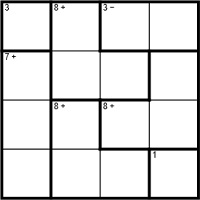
\includegraphics[scale=1]{Gambar/Backtracking1}
\caption[Contoh permainan teka-teki Calcudoku dengan ukuran \textit{grid} 4 x 4 yang belum diselesaikan.  ~\cite{Fahda}]{Contoh permainan teka-teki dengan ukuran \textit{grid} 4 x 4 yang belum diselesaikan.  ~\cite{Fahda}}
\label{fig:backtracking1}
\end{figure}

Untuk menyelesaikan sebuah teka-teki Calcudoku, pemain harus pertama-tama memahami dua permasalahan utama dari teka-teki ini, yaitu:
\begin{enumerate}
\item Angka-angka mana yang harus dimasukkan ke dalam sebuah \textit{cage}
\item Dalam urutan apa angka-angka tersebut harus dimasukkan ke dalam sebuah \textit{cage}
\end{enumerate}

Seperti kebanyakan permainan teka-teki angka, cara yang paling mudah untuk menyelesaikan teka-teki ini adalah dengan mengeliminasi angka-angka yang sudah digunakan dan mencoba satu per satu angka yang mungkin (\textit{trial and error}).

Dalam pengisian teka-teki ini ada dua tahapan, yaitu:
\begin{enumerate}
\item Mencari \textit{cage} yang hanya berukuran 1 sel, karena \textit{cage} ini tidak menghasilkan pertanyaan angka apa dan urutan apa. Tahap ini adalah tahap yang paling jelas. Contoh, pada Gambar~\ref{fig:backtracking1}, \textit{cage} pada sudut kiri atas dan \textit{cage} pada sudut kanan bawah hanya berukuran 1 sel, dan dapat langsung diisi dengan angka tujuannya.
\item Mencari mencari \textit{cage} yang hanya mempunyai satu kemungkinan kombinasi angka, sehingga masalah angka-angka apa yang harus diisi dalam \textit{cage} tersebut terjawab. Contoh, \textit{cage} pada sudut kanan atas mempunyai aturan "3-", artinya angka tujuannya adalah 3 dengan menggunakan operasi pengurangan. Satu-satunya pasangan angka dari himpunan \{1,2,3,4\} yang akan menghasilkan angka 3 saat satu angka dikurangkan dari angka yang lainnya adalah \{1,4\}. Namun masalahnya adalah urutan angka-angka yang harus dimasukkan. Dalam kasus ini, untungnya, sel pada sudut kanan bawah sudah diisi dengan angka 1, maka angka 1 tidak bisa digunakan lagi pada kolom yang paling kanan. Jadi, dengan menggunakan cara eliminasi, sel pada sudut kanan atas harus diisi dengan angka 4 dan sel di sebelah kirinya, yaitu sel pada baris yang paling atas dan kolom ketiga dari kiri, harus diisi dengan angka 1. Hal ini memberikan solusi untuk sel pada baris yang paling atas dan kolom kedua dari kiri, yaitu angka 2, karena angka 2 adalah angka yang belum pernah dipakai dalam baris tersebut. Proses ini berlanjut sampai semua sel dalam \textit{grid} terisi dan menghasilkan solusi pada Gambar~\ref{fig:backtracking2} ~\cite{Fahda}.
\end{enumerate}

\begin{figure}
\centering
\captionsetup{justification=centering}
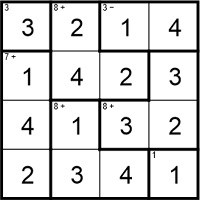
\includegraphics[scale=1]{Gambar/Backtracking2}
\caption[Solusi untuk permainan teka-teki Calcudoku yang diberikan pada Gambar~\ref{fig:backtracking1}  ~\cite{Fahda}]{Solusi untuk permainan teka-teki Calcudoku yang diberikan pada Gambar~\ref{fig:backtracking1}.  ~\cite{Fahda}}
\label{fig:backtracking2}
\end{figure}

Seiring dengan meningkatnya tingkat kesulitan, langkah berikutnya tidak akan langsung muncul dengan jelas. Kadang-kadang, pemain mencapai titik dimana langkah berikutnya tidak pasti. Pemain harus menebak langkah-langkah berikutnya dan melihat apakah langkah ini akan menghasilkan solusinya. Jika tidak, pemain harus mundur kembali ke titik ketidakpastian tersebut.

Sebuah teka-teki Calcudoku dengan ukuran \begin{math}n \times n\end{math}, dengan \begin{math}n\end{math} melambangkan jumlah sel dalam satu baris atau kolom, mempunyai \begin{math}n^2\end{math} sel. Sel yang terletak dalam baris \begin{math}b\end{math} dan kolom \begin{math}k\end{math} diberi label \begin{math}C_{b,k} = bn + k\end{math} dan nilai dari sel tersebut adalah \begin{math}V(C_{b,k}) \in \{1, 2, ..., n\}\end{math}. Sebuah \textit{cage}, yang diberi label \begin{math}A_i\end{math} adalah sebuah himpunan dari sel, yaitu \begin{math}A_i = \{C_{b,k}\}\end{math}. Setiap \textit{cage} terhubung dengan satu operator aritmatika \begin{math}O_i \in \{+, -, \times, \div\}\end{math} dan satu angka tujuan \begin{math}H_i \in N\end{math}. Menurut Johanna, Lukas, dan Saputra, tiga aturan dalam mendefinisikan masalah dalam Calcudoku adalah sebagai berikut ~\cite{JohannaLukasSaputra}:
\begin{enumerate}
\item \begin{math}|A_i| = 1 \rightarrow O_i = \phi\end{math}, artinya setiap \textit{cage} yang jumlah selnya 1 dengan operasi matematika yang terkait dengan \textit{cage} tersebut bersifat homeomorfik (setara).
\item \begin{math}O_i \in {-, \div} \rightarrow |A_i| = 2\end{math}, artinya jika operasi yang digunakan dalam sebuah \textit{cage} adalah pengurangan atau pembagian, maka jumlah sel dalam \textit{cage} tersebut harus 2.
\item \begin{math}\forall C_{b,k} \rightarrow C_{b,k} \in \exists! A_i\end{math}, artinya setiap sel hanya boleh menjadi anggota dari satu dan hanya satu \textit{cage}.
\end{enumerate}
Menurut Johanna, Lukas, dan Saputra, tujuan dari teka-teki ini adalah untuk mencari nilai \begin{math}V(C_{b,k})\end{math} dan memenuhi persyaratan berikut ~\cite{JohannaLukasSaputra}:
\begin{enumerate}
\item \begin{math}|A_i| = 1 \land C_{b,k} \in A_i \rightarrow V(C_{b,k}) = H_i\end{math}, artinya jika sel adalah bagian dari sebuah \textit{cage} yang jumlah selnya 1, maka nilai dari sel tersebut adalah angka tujuan dari \textit{cage} tersebut.
\item \begin{math}O_i \in \{-\} \land A_i = \{C_{a,b}, C_{p,q}\} \rightarrow |V(C_{a,b}) - V(C_{p,q})| = H_i\end{math}, artinya jika sebuah \textit{cage} yang operasi matematikanya adalah pengurangan, maka nilai absolut dari hasil pengurangan nilai kedua sel di dalam \textit{cage} tersebut adalah angka tujuan dari \textit{cage} tersebut.
\item \begin{math}O_i \in \{\div\} \land A_i = \{C_{a,b}, C_{p,q}\} \rightarrow V(C_a,_b) / V(C_{p,q}) = H_i\end{math}, artinya jika sebuah \textit{cage} yang operasi matematikanya adalah pembagian, maka nilai dari hasil pembagian nilai kedua sel di dalam \textit{cage} tersebut adalah angka tujuan dari \textit{cage} tersebut.
\item \begin{math}O_i \in \{+\} \rightarrow \sum_{C_{b,k} \in A_i} V(C_{b,k}) = H_i\end{math}, artinya jika sebuah \textit{cage} yang operasi matematikanya adalah penjumlahan, maka nilai dari hasil penjumlahan dari nilai semua sel di dalam \textit{cage} tersebut adalah angka tujuan dari \textit{cage} tersebut.
\item \begin{math}O_i \in \{\times\} \rightarrow \prod_{C_{b,k} \in A_i} V(C_{b,k}) = H_i\end{math}, artinya jika sebuah \textit{cage} yang operasi matematikanya adalah perkalian, maka nilai dari hasil perkalian dari nilai semua sel di dalam \textit{cage} tersebut adalah angka tujuan dari \textit{cage} tersebut.
\end{enumerate}
		
		\item \textbf{Melakukan studi literatur tentang algoritma \textit{backtracking}.}\\
		{\bf Status :} Ada sejak rencana kerja skripsi.\\
		{\bf Hasil :}
		
		Algoritma \textit{backtracking} adalah sebuah algoritma umum yang mencari solusi dengan mencoba salah satu dari beberapa pilihan, jika pilihan yang dipilih ternyata salah, komputasi dimulai lagi pada titik pilihan dan mencoba pilihan lainnya. Untuk bisa melacak kembali langkah-langkah yang telah dipilih, maka algoritma harus secara eksplisit menyimpan jejak dari setiap langkah yang sudah pernah dipilih, atau menggunakan rekursi (\textit{recursion}). Rekursi dipilih karena jauh lebih mudah daripada harus menyimpan jejak setiap langkah yang pernah dipilih. Hal ini menyebabkan algoritma ini biasanya berbasis DFS (\textit{Depth First Search}).

Algoritma \textit{backtracking} pertama kali diperkenalkan pada tahun 1950 oleh D.H. Lehmer sebagai perbaikan algoritma \textit{brute force}. Algoritma ini lalu dikembangkan lebih lanjut oleh R.J. Walker, S.W. Golomb, dan L.D. Baumert. Algoritma ini terbukti efektif untuk menyelesaikan banyak permainan logika (misalnya \textit{tic tac toe}, \textit{maze}, catur, dan lain-lain) karena algoritma itu terutama berguna untuk menyelesaikan masalah-masalah \textit{constraint satisfaction}, di mana sekumpulan objek harus memenuhi sejumlah batasan.

Menurut Fahda, implementasi algoritma \textit{backtracking} memiliki beberapa sifat umum, yaitu ~\cite{Fahda}:
\begin{enumerate}
\item \textit{Solution space}
\\ Solusi untuk masalah ini dinyatakan sebagai sebuah vektor \begin{math}X\end{math} dengan \textit{\begin{math}n\end{math}-tuple}:
\begin{displaymath}
X = (x_1, x_2, ..., x_n), x_i \in S_i
\end{displaymath}
di mana adalah mungkin bahwa:
\begin{displaymath}
S_1 = S_2 = ... = S_n
\end{displaymath}
\begin{math}n\end{math} adalah jumlah sel dalam satu baris atau kolom. \begin{math}X\end{math} adalah sebuah \textit{tuple} yang berukuran \begin{math}n^2\end{math}, yang mereprentasikan isi dari setiap sel dalam \textit{grid}, dimulai pada sel pada sudut kiri atas, lalu bergerak ke sel di sebelah kanannya dalam baris yang sama, jika sudah mencapai sel yang paling kanan maka bergerak ke sel yang paling kiri pada baris dibawahnya, hingga berakhir di sel pada sudut kanan bawah. \begin{math}S_i\end{math} adalah sebuah himpunan yang berisi angka-angka dari 1 sampai \begin{math}n\end{math}.
\item Fungsi pembangkit \begin{math}X_k\end{math}
\\ Fungsi pembangkit \begin{math}X_k\end{math} dinyatakan sebagai:
\begin{displaymath}
T(k)
\end{displaymath}
di mana \begin{math}T(k)\end{math} membangkitkan nilai \begin{math}X_k\end{math}, dari 1 sampai \begin{math}n\end{math}, yang merupakan komponen dari vektor solusi.
\item Fungsi pembatas
\\ Fungsi pembatas dinyatakan sebagai:
\begin{displaymath}
B(x_1, x_2, ..., x_k)
\end{displaymath}
di mana B bernilai \textit{true} jika \begin{math}(x_1, x_2, ..., x_k)\end{math} mengarah ke solusi. Jika B bernilai \textit{true}, maka nilai \begin{math}x_k+1\end{math} akan terus dibangkitkan, dan jika B bernilai \textit{false}, maka \begin{math}(x_1, x_2, ..., x_k)\end{math} akan dibuang.
\end{enumerate}

Ruang solusi untuk algoritma \textit{backtracking} disusun dalam sebuah struktur berbentuk pohon (\textit{tree}), di mana setiap simpul (\textit{node}) merepresentasikan keadaan masalah dan sisi (\textit{edge}) diberi label \begin{math}x_i\end{math}. Jalur dari akar (\textit{root}) ke daun (\textit{leaf}) merepresentasikan sebuah jawaban yang mungkin, dan semua jalur yang dikumpulkan bersama-sama membentuk ruang solusi. Struktur pohon ini disebut sebagai \textit{state space tree}. Gambar~\ref{fig:backtracking3} menggambarkan contoh sebuah \textit{state space tree}.

\begin{figure}
\centering
\captionsetup{justification=centering}
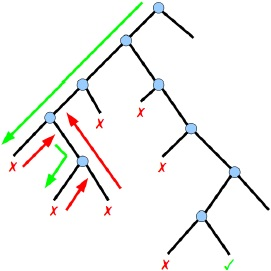
\includegraphics[scale=1]{Gambar/Backtracking3}
\caption[Ilustrasi \textit{state space tree} yang digunakan dalam algoritma  \textit{backtracking}  ~\cite{Fahda}]{Ilustrasi \textit{state space tree} yang digunakan dalam algoritma  \textit{backtracking} ~\cite{Fahda}}
\label{fig:backtracking3}
\end{figure}

Langkah-langkah dalam menggunakan \textit{state space tree} untuk mencari solusi adalah ~\cite{Fahda}:
\begin{enumerate}
\item Solusi dicari dengan membangun jalur dari akar ke daun menggunakan algoritma DFS.
\item Simpul yang terbentuk disebut sebagai simpul hidup (\textit{live nodes}).
\item Simpul yang sedang diperluas disebut sebagai \textit{expand nodes} atau \textit{E-nodes}.
\item Setiap kali sebuah \textit{E-node} sedang diperluas, jalur yang dikembangkannya menjadi lebih panjang.
\item Jika jalur yang sedang dikembangkan tidak mengarah ke solusi, maka \textit{E-node} dimatikan dan menjadi simpul mati (\textit{dead node}).
\item Fungsi yang digunakan untuk mematikan \textit{E-node} adalah implementasi dari fungsi pembatas.
\item Simpul mati tidak akan diperluas.
\item Jika jalur yang sedang dibangun berakhir dengan simpul mati, proses akan mundur ke simpul sebelumnya.
\item Simpul sebelumnya terus membangkitkan simpul anak (\textit{child node}) lainnya, yang kemudian menjadi \textit{E-node} baru.
\item Pencarian selesai jika simpul tujuan tercapai.
\end{enumerate}
Setiap simpul di dalam \textit{state space tree} terkait dengan panggilan rekursif. Jika jumlah simpul di dalam pohon \begin{math}2n\end{math} atau \begin{math}n!\end{math}, maka pada kasus terburuk untuk algoritma \textit{backtracking} ini memiliki kompleksitas waktu \begin{math}O(p(n)2n)\end{math} atau \begin{math}O(q(n)n!)\end{math}, dengan \begin{math}p(n)\end{math} dan \begin{math}q(n)\end{math} sebagai polinomial dengan \begin{math}n\end{math}-derajat menyatakan waktu komputasi untuk setiap simpul.

Algoritma \textit{backtracking} mempunyai beberapa sifat-sifat umum, yaitu ruang solusi (\textit{solution space}), fungsi pembangkit (\textit{generating function}), dan fungsi pembatas (\textit{bounding function}).

Ruang solusi untuk sebuah permainan teka-teki Calcudoku dengan \textit{grid} yang berukuran \begin{math}n \times n\end{math} adalah \begin{math}X = (x_1,x_2,...,x_m), x_i \in \{1,2,...,n\}\end{math}, dengan \begin{math}m = n^2\end{math}. Fungsi pembangkit membangkitkan sebuah integer secara berurutan dari 1 sampai \begin{math}n\end{math} sebagai \begin{math}x_k\end{math}. Fungsi pembatas menggabungkan tiga fungsi pemeriksa pembatas (\textit{constraint checking}), yaitu fungsi pemeriksa kolom (\textit{column checking}), fungsi pemeriksa baris (\textit{row checking}), dan fungsi pemeriksa \textit{grid} (\textit{grid checking}).

Fungsi pemeriksa kolom menghasilkan nilai \textit{true} jika \begin{math}x_k\end{math} belum ada di dalam kolom dan menghasilkan nilai \textit{false} jika \begin{math}x_k\end{math} sudah ada di dalam kolom.

Fungsi pemeriksa baris menghasilkan nilai \textit{true} jika \begin{math}x_k\end{math} belum ada di dalam baris dan menghasilkan nilai \textit{false} jika \begin{math}x_k\end{math} sudah ada di dalam baris.

Fungsi pemeriksa \textit{grid} memeriksa operator pada \textit{grid} dan memeriksa berdasarkan operator yang telah ditentukan. Ada 5 operator yang digunakan dalam fungsi ini, yaitu:

\begin{enumerate}
\item Operator penjumlahan (+), fungsi menghasilkan nilai \textit{true} jika hasil penjumlahan semua nilai yang ada pada \textit{grid} ditambah dengan \begin{math}x_k\end{math} kurang dari atau sama dengan nilai tujuan, dan menghasilkan nilai \textit{false} jika jumlah semua nilai yang ada pada \textit{grid} ditambah \begin{math}x_k\end{math} lebih dari nilai tujuan.
\item Operator pengurangan (-), fungsi menghasilkan nilai \textit{true} jika kedua sel dalam \textit{grid} kosong, atau jika ada satu sel yang kosong dan hasil dari \begin{math}x_k\end{math} dikurangi dengan nilai dari sel yang lainnya atau hasil dari nilai dari sel yang lainnya dikurangi dengan \begin{math}x_k\end{math} menghasilkan nilai tujuan, dan menghasilkan nilai \textit{false} jika ada satu sel kosong dan hasil dari \begin{math}x_k\end{math} dikurangi dengan nilai dari sel yang lainnya atau hasil dari nilai dari sel yang lainnya dikurangi dengan \begin{math}x_k\end{math} tidak menghasilkan nilai tujuan.
\item Operator perkalian (\begin{math}\times\end{math}), fungsi menghasilkan nilai \textit{true} jika hasil perkalian dari semua nilai yang ada pada \textit{grid} dikali dengan \begin{math}x_k\end{math} kurang dari atau sama dengan nilai tujuan, dan menghasilkan nilai \textit{false} jika hasil perkalian dari semua nilai yang ada pada \textit{grid} dikali dengan \begin{math}x_k\end{math} lebih dari nilai tujuan.
\item Operator pembagian (\begin{math}\div\end{math}), fungsi menghasilkan nilai \textit{true} jika kedua sel dalam \textit{grid} kosong, atau jika ada satu sel yang kosong dan hasil dari \begin{math}x_k\end{math} dibagi dengan nilai dari sel yang lainnya atau hasil dari nilai dari sel yang lainnya dibagi dengan \begin{math}x_k\end{math} menghasilkan nilai tujuan, dan menghasilkan nilai \textit{false} jika ada satu sel yang kosong dan hasil dari \begin{math}x_k\end{math} dibagi dengan nilai dari sel yang lainnya atau hasil dari nilai dari sel yang lainnya dibagi dengan \begin{math}x_k\end{math} tidak menghasilkan nilai tujuan.
\item Operator =, fungsi akan menghasilkan nilai \textit{true} jika \begin{math}x_k\end{math} sama dengan nilai tujuan, dan menghasilkan nilai \textit{false} jika \begin{math}x_k\end{math} tidak sama dengan nilai tujuan.
\end{enumerate}

\textit{State space tree} bersifat dinamis, berkembang secara terus-menerus sampai solusi ditemukan. Untuk mengilustrasikan berkembangnya \textit{state space tree}, teka-teki Calcudoku yang digambarkan pada Gambar~\ref{fig:backtracking4} akan digunakan. Berikut ini adalah tahap-tahap berkembangnya \textit{state space tree} untuk teka-teki tersebut.

\begin{figure}
\centering
\captionsetup{justification=centering}
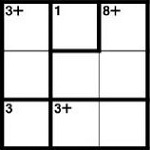
\includegraphics[scale=1]{Gambar/Backtracking4}
\caption[Contoh permainan teka-teki Calcudoku dengan ukuran \textit{grid} 3 x 3 ~\cite{Fahda}]{Contoh permainan teka-teki Calcudoku dengan ukuran \textit{grid} 3 x 3  ~\cite{Fahda}}
\label{fig:backtracking4}
\end{figure}

\begin{enumerate}
\item \textit{State space tree} dimulai dengan \textit{state} 1 yang merepresentasikan sebuah \textit{grid} yang kosong.
\item Fungsi pembangkit pertama-tama akan membangkitkan angka 1 sebagai \begin{math}x_1\end{math}, yang akan diisikan pada sel pertama yang kosong, yaitu sel yang terletak di sudut kiri atas \textit{grid}, atau sel pada kolom ke-1 dan baris ke-1 (\textit{state} 2). Fungsi pembatas akan memeriksa jika langkah ini adalah langkah yang berlaku, dan ternyata langkah ini berlaku.
\item Untuk sel yang kosong berikutnya, yaitu \begin{math}x_2\end{math}, atau sel pada kolom ke-2 dan baris ke-1, fungsi pembangkit akan membangkitkan angka 1 (\textit{state} 3), tetapi langkah ini gagal dalam pemeriksaan baris dalam fungsi pembatas karena angka 1 sudah pernah digunakan pada baris tersebut, ini membentuk sebuah simpul mati.
\item Fungsi pembangkit akan mencoba kemungkinan angka berikutnya, yaitu angka 2 (\textit{state} 4), tetapi langkah ini gagal dalam pemeriksaan \textit{grid} dalam fungsi pembatas karena angka 2 tidak sama dengan angka tujuan, yaitu angka 1.
\item Fungsi pembangkit akan mencoba kemungkinan angka berikutnya, yaitu angka 3 (\textit{state} 5), tetapi langkah ini juga gagal dalam pemeriksaan \textit{grid} dalam fungsi pembatas karena angka 3 tidak sama dengan angka tujuan, yaitu angka 1. Gambar~\ref{fig:backtracking5} menggambarkan \textit{state} 3, \textit{state} 4, dan \textit{state} 5 dalam penyelesaian teka-teki Calcudoku ini.

\begin{figure}
\centering
\captionsetup{justification=centering}
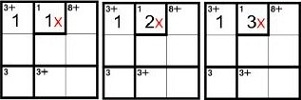
\includegraphics[scale=1]{Gambar/Backtracking5}
\caption[Ilustrasi \textit{state} 3, 4, dan 5 pada sebuah \textit{grid} teka-teki Calcudoku ~\cite{Fahda}]{Ilustrasi \textit{state} 3, 4, dan 5 pada sebuah \textit{grid} teka-teki Calcudoku  ~\cite{Fahda}}
\label{fig:backtracking5}
\end{figure}

\item Karena tidak ada solusi yang mungkin, maka algoritma \textit{backtracking} akan mundur ke \textit{state} 1. Fungsi pembangkit akan membangkitkan kemungkinan angka berikutnya sebagai \begin{math}x_1\end{math}, yaitu 2, dan ternyata angka 2 berlaku sebagai \begin{math}x_1\end{math} (\textit{state} 6), sehingga algoritma bisa maju ke \begin{math}x_2\end{math}, yaitu sel pada kolom ke-2 dan baris ke-1.
\item Fungsi pembangkit akan membangkitkan angka 1 (\textit{state} 7), dan ini memenuhi syarat yang ditentukan dalam fungsi pembatas, karena angka 1 sama dengan angka tujuan, yaitu angka 1, sehingga algoritma bisa maju ke \begin{math}x_3\end{math}, yaitu sel pada kolom ke-3 dan baris ke-1.
\item Angka 1 (\textit{state} 8) gagal dalam pemeriksaan baris karena angka 1 sudah pernah digunakan pada baris tersebut.
\item Angka 2 (\textit{state} 9) juga gagal dalam pemeriksaan baris karena angka 2 sudah pernah digunakan pada baris tersebut.
\item Hal ini menyebabkan hanya tersisa angka 3 sebagai angka yang bisa dimasukkan ke dalam \begin{math}x_3\end{math} (\textit{state} 10). Karena \textit{state} 10 ternyata berlaku, maka algoritma telah selesai mengisi baris ke-1, dan akan mulai mengisi baris ke-2.
\item Algoritma lalu membuat \textit{state} baru dengan mengisikan angka 1 pada \begin{math}x_4\end{math}, yaitu sel pada kolom ke-1 dan baris ke-2 (\textit{state} 11). Ini memenuhi pemeriksaan pembatas, karena 2 + 1 = 3, sehingga algoritma akan maju ke sel berikutnya, yaitu \begin{math}x_5\end{math}, atau sel pada kolom ke-2 dan baris ke-2.
\item Angka 1 (\textit{state} 12) jelas tidak bisa digunakan karena gagal dalam pemeriksaan kolom dan pemeriksaan baris; angka 1 sudah pernah digunakan pada kolom dan baris tersebut.
\item Angka 2 (\textit{state} 13) adalah langkah yang berlaku, sehingga algoritma bisa maju ke sel berikutnya, yaitu \begin{math}x_6\end{math}, atau sel pada kolom ke-3 dan baris ke-2.
\item Algoritma mengisikan \begin{math}x_6\end{math} dengan angka 1 (\textit{state} 14), tetapi gagal dalam pemeriksaan baris karena angka 1 sudah pernah digunakan pada baris tersebut.
\item Algoritma lalu mencoba kemungkinan angka berikutnya, yaitu angka 2 (\textit{state} 15), tetapi juga gagal dalam pemeriksaan baris karena angka 2 sudah pernah digunakan pada baris tersebut.
\item Algoritma lalu mencoba kemungkinan angka berikutnya, yaitu angka 3 (\textit{state} 16), tetapi juga gagal, kali ini angka 3 gagal dalam pemeriksaan kolom karena angka 3 sudah pernah digunakan pada kolom tersebut.
\item Karena semua kemungkinan angka gagal dalam pemeriksaan baris dan kolom, maka algoritma akan mundur ke \textit{state} 11 dan mencoba kemungkinan angka berikutnya, yaitu angka 3 (\textit{state} 17), dan ternyata angka 3 berlaku sebagai \begin{math}x_5\end{math}, sehingga algoritma bisa maju ke sel berikutnya, yaitu \begin{math}x_6\end{math}.
\item Algoritma lalu mencoba angka 1 (\textit{state} 18) sebagai \begin{math}x_6\end{math}, tetapi gagal dalam pemeriksaan baris karena angka 1 sudah pernah digunakan dalam baris tersebut.
\item Algoritma lalu mencoba kemungkinan angka berikutnya, yaitu angka 2 (\textit{state} 19), dan ternyata angka 2 berlaku. Algoritma telah selesai mengisi baris ke-2. Gambar~\ref{fig:backtracking6} menggambarkan \textit{state} 19 dalam penyelesaian teka-teki Calcudoku ini.

\begin{figure}
\centering
\captionsetup{justification=centering}
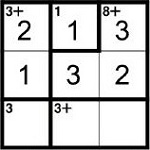
\includegraphics[scale=1]{Gambar/Backtracking6}
\caption[Ilustrasi \textit{state} 19 pada sebuah \textit{grid} teka-teki Calcudoku ~\cite{Fahda}]{Ilustrasi \textit{state} 19 pada sebuah \textit{grid} teka-teki Calcudoku  ~\cite{Fahda}}
\label{fig:backtracking6}
\end{figure}

\item Algoritma mulai mengisikan sel-sel yang terletak pada baris ke-3. Algoritma mengisi dari kolom yang paling kiri ke kolom yang paling kanan. Algoritma mengisikan \begin{math}x_7\end{math}, yaitu sel pada kolom ke-1 dan baris ke-3 dengan angka 1 (\textit{state} 20), tetapi gagal dalam pemeriksaan kolom, karena angka 1 sudah pernah digunakan dalam kolom tersebut.
\item Algoritma lalu mencoba kemungkinan angka berikutnya, yaitu angka 2 (\textit{state} 21), tetapi juga gagal dalam pemeriksaan kolom, karena angka 2 sudah pernah digunakan dalam kolom tersebut.
\item Algoritma lalu mencoba kemungkinan angka berikutnya, yaitu angka 3 (\textit{state} 22), dan ternyata berhasil, sehingga algoritma bisa maju ke sel berikutnya, yaitu \begin{math}x_8\end{math}, atau sel pada kolom ke-2 dan baris ke-3.
\item Algoritma lalu mencoba mengisikan angka 1 pada \begin{math}x_8\end{math} (\textit{state} 23), tetapi gagal dalam pemeriksaan kolom, karena angka 1 sudah pernah digunakan dalam kolom tersebut.
\item Algoritma lalu mencoba kemungkinan angka berikutnya, yaitu angka 2 (\textit{state} 24), dan ternyata berhasil, sehingga algoritma bisa maju ke sel berikutnya, yaitu \begin{math}x_9\end{math}, atau sel pada kolom ke-3 dan baris ke-3.
\item \begin{math}x_9\end{math} adalah sel terakhir, terletak pada sudut kanan bawah \textit{grid}. Algoritma lalu mencoba mengisikan \begin{math}x_9\end{math} dengan angka 1 (\textit{state} 25), dan ternyata berhasil. Algoritma telah selesai mengisikan seluruh sel dalam \textit{grid} dengan benar. Gambar~\ref{fig:backtracking7} menggambarkan \textit{state} 25 dalam penyelesaian teka-teki Calcudoku ini. Algoritma ini mencapai solusinya pada \textit{state} 25, seperti pada \textit{state space tree} yang digambarkan dalam Gambar~\ref{fig:backtracking8}. \textit{State space tree} ini telah mencapai simpul tujuannya, yaitu simpul 25, dengan jalur 2-1-3-1-3-2-3-2-1.

\begin{figure}
\centering
\captionsetup{justification=centering}
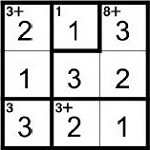
\includegraphics[scale=1]{Gambar/Backtracking7}
\caption[\textit{State} 25, simpul tujuan, sebagai hasil yang dicapai  ~\cite{Fahda}]{\textit{State} 25, simpul tujuan, sebagai hasil yang dicapai  ~\cite{Fahda}}
\label{fig:backtracking7}
\end{figure}

\end{enumerate}

\begin{figure}
\centering
\captionsetup{justification=centering}
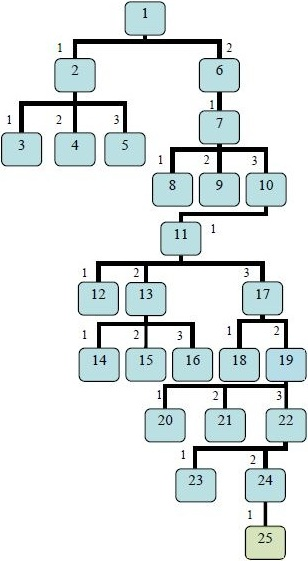
\includegraphics[scale=1]{Gambar/Backtracking8}
\caption[\textit{state space tree} yang dikembangkan dalam proses menyelesaikan teka-teki Calcudoku yang digambarkan pada  Gambar~\ref{fig:backtracking4}  ~\cite{Fahda}]{\textit{state space tree} yang dikembangkan dalam proses menyelesaikan teka-teki Calcudoku yang digambarkan pada  Gambar~\ref{fig:backtracking4}  ~\cite{Fahda}}
\label{fig:backtracking8}
\end{figure}

Tinggi pohon yang dikembangkan untuk menyelesaikan sebuah teka-teki dengan ukuran \begin{math}n \times n\end{math} seharusnya memiliki tinggi \begin{math}n^2+1\end{math} saat mencapai simpul tujuannya, dengan jalur dari simpul akar ke simpul tujuan merepresentasikan semua angka yang digunakan untuk mengisi \textit{grid} dari sel pada sudut kiri atas ke sel pada sudut kanan bawah.

Singkatnya, langkah-langkah dasar dari implementasi algoritma \textit{backtracking} dapat dijelaskan sebagai berikut ~\cite{Fahda}:
\begin{enumerate}
\item Carilah sel pertama atau sel yang kosong di dalam \textit{grid}.
\item Isilah sel dengan sebuah angka dimulai dari 1 sampai \begin{math}n\end{math} sampai sebuah angka yang berlaku (\textit{valid}) ditemukan atau sampai angka sudah melebihi \begin{math}n\end{math}.
\item Jika angka untuk sel berlaku, ulangi langkah 1 dan 2.
\item Jika angka untuk sel sudah melebihi \begin{math}n\end{math} dan tidak ada angka dari 1 sampai \begin{math}n\end{math} yang berlaku untuk sel tersebut, mundur ke sel sebelumnya dan cobalah kemungkinan angka berikutnya yang berlaku untul sel tersebut.
\item Jika tidak ada lagi sel yang kosong, solusi sudah ditemukan.
\end{enumerate}
		
		\item \textbf{Melakukan studi literatur tentang algoritma \textit{hybrid genetic}.}\\
		{\bf Status :} Ada sejak rencana kerja skripsi.\\
		{\bf Hasil :}
		
		Dalam kasus ini, algoritma \textit{hybrid genetic} adalah gabungan dari algoritma \textit{rule based} dan algoritma genetik. Algoritma \textit{rule based} akan dijalankan sampai pada titik dimana algoritma tidak bisa menyelesaikan permainan teka-teki Calcudoku. Jika algoritma sudah tidak bisa menyelesaikan permainan, maka algoritma genetik akan mulai dijalankan.

\textbf{Algoritma \textit{Rule Based}} \\

Algoritma \textit{rule based} adalah sebuah algoritma berbasis aturan logika untuk menyelesaikan teka-teki Sudoku dan variasinya, termasuk Calcudoku. Menurut Johanna, Lukas, dan Saputra, beberapa aturan logika yang digunakan dalam algoritma ini adalah \textit{single square rule}, \textit{naked subset rule}, \textit{hidden single rule}, \textit{evil twin rule}, \textit{killer combination}, dan \textit{X-wing} ~\cite{JohannaLukasSaputra}.

Aturan \textit{single square} digunakan jika sebuah \textit{cage} hanya berisi satu sel. Hal ini berarti nilai dari sel tersebut sama dengan angka tujuan yang telah ditentukan.

Aturan \textit{naked subset} digunakan jika ada \begin{math}n\end{math} sel dalam kolom atau baris yang sama yang mempunyai \begin{math}n\end{math} kemungkinan nilai yang sama persis untuk mengisikannya, dengan \begin{math}n \geq 2 \end{math}. Hal ini berarti sel-sel lainnya dalam baris dan kolom tersebut tidak mungkin diisi dengan nilai yang sama dengan nilai milik \begin{math}n\end{math} sel tersebut. Gambar~\ref{fig:hybrid2} menunjukkan bagaimana cara kerja aturan ini. Sel-sel pada kolom ke-4 dan ke-6 mempunyai tepat dua kemungkinan nilai (1 atau 7). Ini disebut sebagai \textit{naked pair}. Karena angka 1 dan 7 harus diisi pada sel-sel pada kolom ke-4 dan ke-6, maka angka 1 dan 7 bisa dieliminasi dari sel-sel pada kolom ke-7 dan ke-8.

\begin{figure}
\centering
\captionsetup{justification=centering}
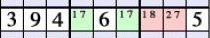
\includegraphics[scale=1]{Gambar/HybridGenetic2}
\caption[Contoh bagaimana cara mendeteksi aturan  \textit{naked pair}  ~\cite{JohannaLukasSaputra}]{Contoh bagaimana cara mendeteksi aturan  \textit{naked pair}  ~\cite{JohannaLukasSaputra}}
\label{fig:hybrid2}
\end{figure}

Aturan \textit{evil twin} digunakan jika sebuah \textit{cage} berisikan dua sel, dan salah satu dari kedua sel sudah terisi, maka sel yang satunya lagi diisi dengan angka yang jika kedua angka dihitung dengan operasi matematika yang ditentukan maka akan menghasilkan angka tujuan yang ditentukan. Aturan ini adalah aturan yang paling mudah. Kenyataannya, aturan ini bisa digeneralisasikan untuk \textit{cage} yang berukuran lebih dari 2 sel. Sel yang belum terisi yang terakhir dalam sebuah area diisi oleh sebuah nilai yang diperlukan untuk mencapai nilai tujuan menggunakan operasi matematika yang telah ditentukan. Contohnya, pada Gambar~\ref{fig:hybrid3}, begitu sel di sudut kiri bawah diisi oleh angka 4, maka sel diatasnya harus diisi oleh angka 9.

\begin{figure}
\centering
\captionsetup{justification=centering}
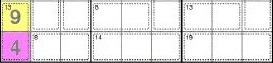
\includegraphics[scale=1]{Gambar/HybridGenetic3}
\caption[Contoh aturan  \textit{evil twin}  ~\cite{JohannaLukasSaputra}]{Contoh aturan  \textit{evil twin}  ~\cite{JohannaLukasSaputra}}
\label{fig:hybrid3}
\end{figure}

Aturan \textit{hidden single} digunakan jika sebuah angka hanya bisa diisikan dalam satu sel dalam sebuah baris atau kolom. Aturan ini secara konsep cukup mudah, tetapi kadang-kadang sulit untuk diamati. Pada Gambar~\ref{fig:hybrid4}, nilai-nilai yang mungkin untuk sel yang paling kiri adalah 3, 5, dan 7, tetapi dalam baris ini, angka 7 harus muncul dalam salah satu selnya, dan hanya sel yang paling kiri tersebut yang memiliki kemungkinan nilai 7. Ini disebut sebagai \textit{hidden single}. Sel tersebut harus diisi dengan angka 7.

\begin{figure}
\centering
\captionsetup{justification=centering}
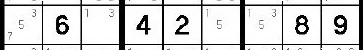
\includegraphics[scale=1]{Gambar/HybridGenetic4}
\caption[Contoh aturan  \textit{hidden single}  ~\cite{JohannaLukasSaputra}]{Contoh aturan  \textit{hidden single}  ~\cite{JohannaLukasSaputra}}
\label{fig:hybrid4}
\end{figure}

Aturan \textit{killer combination} adalah aturan yang paling krusial. Aturan ini digunakan jika sebuah \textit{cage} berisikan sel-sel yang berada dalam baris atau kolom yang sama dan operasi yang ditentukan adalah penjumlahan. Kemungkinan angka yang unik untuk aturan \textit{killer combination} berhubungan dengan ukuran \textit{cage}. Contoh, jika sebuah \textit{cage} memiliki dua sel dan angka tujuannya adalah 3, maka kemungkinan angka yang bisa diisikan ke dalam kedua sel tersebut adalah 1 atau 2. Hal ini berarti semua angka lainnya tidak mungkin diisikan ke dalam kedua sel tersebut. Contoh lain, jika sebuah \textit{cage} memiliki tiga sel dan angka tujuannya adalah 24, maka kemungkinan angka yang bisa diisikan ke dalam ketiga sel tersebut adalah 7, 8, atau 9. Gambar~\ref{fig:hybrid5} menampilkan contoh penerapan aturan \textit{killer combination} untuk \textit{cage} dengan ukuran 2 sel. Tabel ini juga bisa diperluas untuk ukuran \textit{cage} lainnya.

\begin{figure}
\centering
\captionsetup{justification=centering}
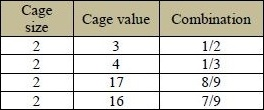
\includegraphics[scale=1]{Gambar/HybridGenetic5}
\caption[Contoh aturan  \textit{killer combination} untuk \textit{cage} dengan ukuran 2 sel  ~\cite{JohannaLukasSaputra}]{Contoh aturan  \textit{killer combination} untuk \textit{cage} dengan ukuran 2 sel ~\cite{JohannaLukasSaputra}}
\label{fig:hybrid5}
\end{figure}

Aturan \textit{X-wing} digunakan jika hanya ada dua kemungkinan angka yang bisa diisikan ke dalam dua sel yang berada di dalam dua baris yang berbeda, dan dua kemungkinan angka tersebut juga berada di dalam kolom yang sama maka sel-sel lainnya dalam kolom tersebut tidak mungkin diisi oleh dua kemungkinan angka tersebut, atau jika hanya ada dua kemungkinan angka yang bisa diisikan ke dalam dua sel yang berada di dalam dua kolom yang berbeda, dan dua kemungkinan angka tersebut juga berada di dalam baris yang sama maka sel-sel lainnya dalam baris tersebut tidak mungkin diisi oleh dua kemungkinan angka tersebut. Gambar~\ref{fig:hybrid6} menampilkan contoh penggunaan aturan \textit{X-wing}. Misalnya, jika sel A diisi oleh angka 7, maka angka 7 akan dieliminasi dari sel B dan sel C. Karena sel A dengan sel C dan sel D 'terkunci', maka sel D harus diisi oleh angka 7. Jadi, angka 7 harus di isi pada sel A dan sel D atau pada sel B dan sel C. Angka 7 bisa dieliminasi dari sel-sel yang berwarna hijau.

\begin{figure}
\centering
\captionsetup{justification=centering}
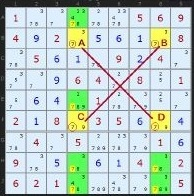
\includegraphics[scale=1]{Gambar/HybridGenetic6}
\caption[Contoh aturan  \textit{X-wing}  ~\cite{JohannaLukasSaputra}]{Contoh aturan  \textit{X-wing} ~\cite{JohannaLukasSaputra}}
\label{fig:hybrid6}
\end{figure}

\textbf{Algoritma Genetik} \\

Pencarian heuristik adalah sebuah teknik pencarian kecerdasan buatan (\textit{artifical intelligence}) yang menggunakan heuristik dalam langkah-langkahnya. Heuristik adalah semacam aturan tidak tertulis yang mungkin menghasilkan solusi. Heuristik kadang-kadang efektif, tetapi tidak dijamin akan berhasil. dalam setiap kasus. Heuristik memerankan peran penting dalam strategi pencarian karena sifat eksponensial dari kebanyakan masalah. Heuristik membantu mengurangi jumlah alternatif solusi dari angka yang bersifat eksponensial menjadi angka yang bersifat polinomial. Contoh teknik pencarian heuristik adalah \textit{Generate and Test}, \textit{Hill Climbing}, dan \textit{Best First Search}.

Algoritma genetik adalah salah satu teknik heuristik \textit{Generate and Test} yang terinspirasi oleh sistem seleksi alam. Algoritma ini adalah perpaduan dari bidang biologi dan ilmu komputer. Algoritma ini adalah salah satu dari teknik pencarian heuristik.

Algoritma genetik adalah salah satu teknik heuristik \textit{Generate and Test} yang terinspirasi oleh sistem seleksi alam. Algoritma ini adalah perpaduan dari bidang biologi dan ilmu komputer. Algoritma ini memanipulasi informasi, biasanya disebut sebagai kromosom. Kromosom ini meng-\textit{encode} kemungkinan jawaban untuk sebuah masalah yang diberikan. Kromosom dievaluasi dan diberi \textit{fitness value} berdasarkan seberapa baikkah kromosom dalam menyelesaikan masalah yang diberikan berdasarkan kriteria yang ditentukan oleh pembuat program. Nilai kelayakan ini digunakan sebagai probabilitas kebertahanan hidup kromosom dalam satu siklus reproduksi. Kromosom baru (kromosom anak, \textit{child chromosome}) diproduksi dengan menggabungkan dua (atau lebih) kromosom orang tua (\textit{parent chromosome}). Proses ini dirancang untuk menghasilkan kromosom-kromosom keturunan yang lebih layak, kromosom-kromosom ini menyandikan jawaban yang lebih baik, sampai solusi yang baik dan yang bisa diterima ditemukan.

Cara kerja algoritma genetik adalah sebagai berikut ~\cite{JohannaLukasSaputra}:
\begin{enumerate}
\item Menentukan populasi kromosom kemungkinan jawaban awal.
\item Membangkitkan populasi kemungkinan jawaban awal secara acak.
\item Mengevaluasi fungsi objektif.
\item Melakukan operasi terhadap kromosom menggunakan operator genetik (reproduksi, kawin silang, dan mutasi).
\item Ulangi langkah 3 dan 4 sampai mencapai kriteria untuk menghentikan algoritma.
\end{enumerate}
Langkah-langkah utama dalam penggunaan algoritma genetik adalah membangkitkan populasi kemungkinan jawaban, mencari fungsi objektif dan fungsi kelayakan, dan penggunaan operator genetik.

\textbf{Algoritma \textit{Hybrid Genetic}} \\

Pencarian \textit{rule based} dimulai dengan mengasumsikan semua nilai sel yang tidak diketahui dengan semua kemungkinan nilai untuk mengisi sel tersebut tanpa melanggar batasan, dengan \begin{math}P(C_{b,k}) = {1, 2, ..., n}\end{math}. Setelah nilai dari satu sel sudah ditentukan, kemungkinan nilai untuk beberapa sel tertentu diperbaharui. Misalnya, penggunaan aturan \textit{naked single} yang dinyatakan dalam persamaan 1 di bawah ini, akan mengakibatkan semua kemungkinan nilai untuk semua sel lain dalam baris yang sama dan dalam kolom yang sama harus diperbaharui, seperti dinyatakan dalam persamaan 2 dan 3 di bawah ini. Aturan \textit{naked pair}, salah satu dari aturan jenis \textit{naked subset}, dinyatakan dalam persamaan 4 untuk baris dan persamaan 5 untuk kolom. ~\cite{JohannaLukasSaputra}

\begin{enumerate}
\item \begin{math}|P(C_{b,k})| = 1 \land x \in P(C_{b,k}) \rightarrow V(C_{b,k}) = x\end{math}, artinya jika sebuah \textit{cage} berukuran 1 sel, dan \begin{math}x\end{math} adalah nilai tujuan dari \textit{cage} tersebut, maka nilai dari sel tersebut adalah \begin{math}x\end{math}.
\item \begin{math}(V(C_{b,k}) = x) \land (\forall a \in \{1, 2, ..., n\}) \rightarrow P(C_{a,k}) = P(C_{a,k}) - \{x\}\end{math}, artinya jika nilai suatu sel pada baris \begin{math}b\end{math} dan kolom \begin{math}k\end{math} adalah \begin{math}x\end{math}, maka \begin{math}x\end{math} dihapus dari kemungkinan angka-angka yang bisa digunakan untuk mengisi sel-sel lain pada baris \begin{math}b\end{math}.
\item \begin{math}(V(C_{b,k}) = x) \land (\forall q \in \{1, 2, ..., n\}) \rightarrow P(C_{b,q}) = P(C_{b,q}) - \{x\}\end{math} artinya jika nilai suatu sel pada baris \begin{math}b\end{math} dan kolom \begin{math}k\end{math} adalah \begin{math}x\end{math}, maka \begin{math}x\end{math} dihapus dari kemungkinan angka-angka yang bisa digunakan untuk mengisi sel-sel lain pada kolom \begin{math}k\end{math}.
\item \begin{math}|P(C_{b,k1})| = |P(C_{b,k2})| = 2 \land P(C_{b,k1}) = P(C_{b,k2}) \rightarrow P(C_{b,q}) = P(C_{b,q}) - P(C_{b,k1})\end{math}, artinya jika ada dua sel dalam satu baris yang hanya bisa diisi oleh dua kemungkinan angka, maka kedua angka tersebut dihapus dari kemungkinan angka-angka yang bisa digunakan untuk mengisi sel-sel lain pada baris tersebut.
\item \begin{math}|P(C_{b1,k})| = |P(C_{b2,k})| = 2 \land P(C_{b1,k}) = P(C_{b2,k}) \rightarrow P(C_{p,k}) = P(C_{p,k}) - P(C_{b1,k})\end{math}, artinya jika ada dua sel dalam satu kolom yang hanya bisa diisi oleh dua kemungkinan angka, maka kedua angka tersebut dihapus dari kemungkinan angka-angka yang bisa digunakan untuk mengisi sel-sel lain pada kolom tersebut.
\end{enumerate}

Algoritma genetik digunakan saat teka-teki masih tidak bisa diselesaikan setelah mengerjakan semua aturan logika secara berulang-ulang. Algoritma ini dimulai dengan meng-\textit{encode} kromosom. Satu kromosom terdiri dari \begin{math}k\end{math} segmen, dengan \begin{math}m \leq n\end{math}. Satu segmen berisikan sekumpulan gen yang belum diselesaikan yang berada di dalam segmen tersebut. Sebuah segmen merepresentasikan sebuah baris atau kolom. Dalam sebuah kromosom, segmen diurutkan dari baris yang paling atas ke baris yang paling bawah atau dari kolom yang paling kiri ke kolom yang paling kanan. Contoh, salah satu kromosom dari permainan teka-teki Calcudoku pada Gambar~\ref{fig:hybrid8} adalah: \begin{displaymath}34 \ 35 \ | \ 28 \ 29 \ 24 \ 25 \ | \ 0 \ 4 \ 5 \ 1 \ 2 \ 3 \ | \ 11 \ 6 \ 9 \ 7 \ 8 \ 10 \ | \ 12 \ 14 \ 15 \ 17 \ 16 \ 13 \ | \ 20 \ 18 \ 19 \ 23 \ 21 \ 22\end{displaymath} Setiap segmen dalam contoh kromosom ini merepresentasikan sebuah baris yang belum terselesaikan.

\begin{figure}
\centering
\captionsetup{justification=centering}
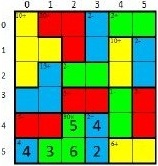
\includegraphics[scale=1]{Gambar/HybridGenetic8}
\caption[Contoh permainan teka-teki Calcudoku dengan ukuran \textit{grid} 6 x 6~\cite{JohannaLukasSaputra}]{Contoh permainan teka-teki Calcudoku dengan ukuran \textit{grid} 6 x 6 ~\cite{JohannaLukasSaputra}}
\label{fig:hybrid8}
\end{figure}

Menurut Johanna, Lukas, dan Saputra, fungsi objektif, yang direpresentasikan dengan \begin{math}x_j\end{math}, akan dihitung setelah pembangkitan nilai dari gen pada kromosom sudah dilakukan. Nilai untuk gen ke-\begin{math}j\end{math} pada sebuah kromosom direpresentasikan dengan \begin{math}w_j\end{math}. \begin{math}x_j\end{math} akan bernilai 0 jika belum diselesaikan (\begin{math}w_j = 0\end{math}), dan bernilai 1 jika sudah diselesaikan (\begin{math}w_j \neq 0\end{math}). Untuk kromosom dengan jumlah gen \begin{math}k\end{math}, fungsi kelayakan, yaitu hasil penjumlahan dari hasil fungsi objektif untuk setiap gen dibagi dengan jumlah gen, dinyatakan dalam persamaan di bawah ini ~\cite{JohannaLukasSaputra}:
\begin{displaymath}
x_j =
\begin{cases}
0, w_j = 0 \\
1, w_j \neq 0
\end{cases}
\end{displaymath}
\begin{displaymath}
fitness = \frac{\sum_{j=0}^k x_j}{k}
\end{displaymath}
Jadi, solusi dari teka-teki ini adalah mencari kromosom yang nilai kelayakannya 1.

Dalam proses reproduksi kawin silang, dua kromosom, yaitu kromosom orang tua, disilangkan untuk membuat dua kromosom yang baru, yaitu kromosom anak, dengan metodologi kawin silang \textit{\begin{math}N\end{math}-segments}. Gambar~\ref{fig:hybrid9} menggambarkan contoh proses kawin silang antara dua kromosom.

\begin{figure}
\centering
\captionsetup{justification=centering}
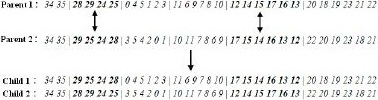
\includegraphics[scale=1]{Gambar/HybridGenetic9}
\caption[Contoh proses kawin silang antara dua kromosom ~\cite{JohannaLukasSaputra}]{Contoh proses kawin silang antara dua kromosom ~\cite{JohannaLukasSaputra}}
\label{fig:hybrid9}
\end{figure}

Pertukaran mutasi digunakan untuk mendapatkan kemungkinan kromosom yang lain. Mutasi dilakukan di antara gen yang berada dalam segmen yang sama. Gambar~\ref{fig:hybrid10} adalah contoh proses mutasi antara dua gen dalam segmen yang sama.

\begin{figure}
\centering
\captionsetup{justification=centering}
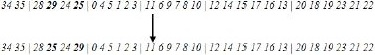
\includegraphics[scale=1]{Gambar/HybridGenetic10}
\caption[Contoh proses mutasi ~\cite{JohannaLukasSaputra}]{Contoh proses mutasi ~\cite{JohannaLukasSaputra}}
\label{fig:hybrid10}
\end{figure}

Cara kerja algoritma \textit{hybrid genetic} menurut Johanna, Lukas, dan Saputra adalah sebagai berikut ~\cite{JohannaLukasSaputra}:
\begin{enumerate}
\item Masukkan teka-teki yang akan diselesaikan sebagai input.
\item Program akan merepresentasikan input yang dimasukkan dalam format teka-teki.
\item Program akan mencoba menyelesaikan teka-teki tersebut dengan menggunakan algoritma \textit{rule based} terlebih dahulu.
\item Jika program berhasil menyelesaikan teka-teki tersebut dengan menggunakan algoritma \textit{rule based}, maka algoritma selesai.
\item Jika program gagal dengan menggunakan algoritma \textit{rule based}, maka program akan mencoba menyelesaikan teka-teki tersebut dengan menggunakan algoritma genetik.
\item Jika program berhasil menyelesaikan teka-teki tersebut dengan menggunakan algoritma genetik, maka algoritma selesai.
\item Jika program gagal dalam menyelesaikan teka-teki tersebut setelah menggunakan algoritma genetik, artinya algoritma gagal dalam menyelesaikan teka-teki terseebut.
\end{enumerate}
Alur (\textit{flow chart}) penyelesaian permainan teka-teki Calcudoku dengan menggunakan algoritma \textit{hybrid genetic} dapat dilihat di Gambar~\ref{fig:hybrid7}.

\begin{figure}
\centering
\captionsetup{justification=centering}
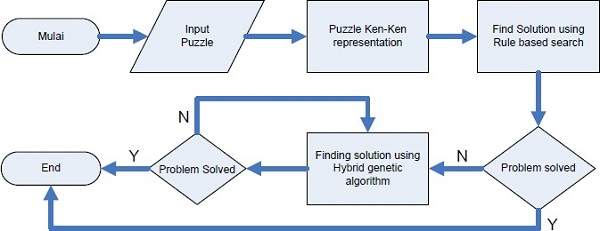
\includegraphics[scale=1]{Gambar/HybridGenetic7}
\caption[Alur penyelesaian permainan teka-teki Calcudoku dengan menggunakan algoritma \textit{hybrid genetic} ~\cite{JohannaLukasSaputra}]{Alur penyelesaian permainan teka-teki Calcudoku dengan menggunakan algoritma \textit{hybrid genetic} ~\cite{JohannaLukasSaputra}}
\label{fig:hybrid7}
\end{figure}

		\item \textbf{Melakukan analisis dan menentukan fitur-fitur yang diperlukan dalam perangkat lunak permainan teka-teki Calcudoku.}\\
		{\bf Status :} Dihapus atau tidak dikerjakan\\
		{\bf Hasil :} Diganti dengan poin berikutnya, yaitu melakukan analisis cara kerja algoritma \textit{backtracking} dan algoritma \textit{hybrid genetic} untuk Calcudoku.
						
		\item \textbf{Melakukan analisis cara kerja algoritma \textit{backtraccking} dan algoritma \textit{hybrid genetic} untuk Calcudoku.}\\
		{\bf Status :} Baru ditambahkan setelah UTS Skripsi 1.\\
		{\bf Hasil :}
		
		\textbf{Algoritma \textit{Backtracking}}
		
		Untuk mengilustrasikan cara kerja algoritma \textit{backtracking}, akan digunakan permainan teka-teki Calcudoku yang digambarkan pada Gambar~\ref{fig:analisisbt1} sebagai contoh.

\begin{figure}
\centering
\captionsetup{justification=centering}
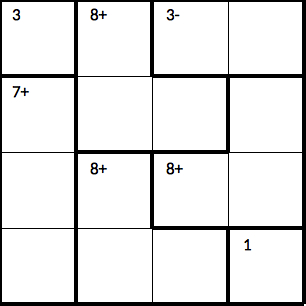
\includegraphics[scale=0.333]{Gambar/backtracking/State1}
\caption[Contoh permainan teka-teki Calcudoku dengan ukuran \textit{grid} 4 x 4 yang belum diselesaikan, seperti yang digambarkan pada Gambar~\ref{fig:backtracking1}.  ~\cite{Fahda}]{Contoh permainan teka-teki dengan ukuran \textit{grid} 4 x 4 yang belum diselesaikan, seperti yang digambarkan pada Gambar~\ref{fig:backtracking1}.  ~\cite{Fahda}}
\label{fig:analisisbt1}
\end{figure}

\begin{itemize}
\item Algoritma \textit{backtracking} dimulai dengan teka-teki yang belum diselesaikan, seperti yang digambarkan pada Gambar~\ref{fig:analisisbt1} (\textit{state} 1).
\item Algoritma mengisikan sel pada baris ke-1 dan kolom ke-1 dengan angka 1 (\textit{state} 2), tetapi angka 1 tidak sesuai dengan angka tujuan dari \textit{cage} tersebut.
\item Algoritma lalu mencoba kemungkinan angka berikutnya, yaitu angka 2 (\textit{state} 3), tetapi angka 2 juga tidak sesuai dengan angka tujuan dari \textit{cage} tersebut.
\item Algoritma lalu mencoba kemungkinan angka berikutnya, yaitu angka 3 (\textit{state} 4), seperti dapat dilihat pada Gambar~\ref{fig:analisisbt2}, dan ternyata angka 3 sesuai dengan angka tujuan dari \textit{cage} tersebut, sehingga algoritma dapat maju ke sel berikutnya.

\begin{figure}
\centering
\captionsetup{justification=centering}
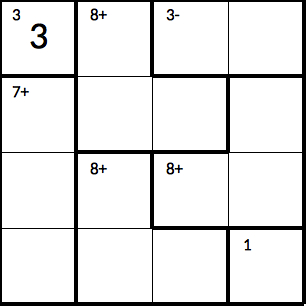
\includegraphics[scale=0.333]{Gambar/backtracking/State4}
\caption[\textit{State} 4]{\textit{State} 4}
\label{fig:analisisbt2}
\end{figure}

\item Algoritma lalu mengisikan sel pada baris ke-1 dan kolom ke-2 dengan angka 1 (\textit{state} 5). Algoritma lalu maju ke sel berikutnya.
\item Algoritma lalu mengisikan sel pada baris ke-1 dan kolom ke-3 dengan angka 1 (\textit{state} 6), tetapi angka 1 sudah pernah digunakan dalam baris tersebut.
\item Algoritma lalu mencoba kemungkinan angka berikutnya, yaitu angka 2 (\textit{state} 7). Algoritma lalu maju ke sel berikutnya.
\item Algoritma lalu mengisikan sel pada baris ke-1 dan kolom ke-4 dengan angka 1 (\textit{state} 8), tetapi angka 1 sudah pernah digunakan dalam baris tersebut.
\item Algoritma lalu mencoba kemungkinan angka berikutnya, yaitu angka 2 (\textit{state} 9), tetapi angka 2 sudah pernah digunakan dalam baris tersebut.
\item Algoritma lalu mencoba kemungkinan angka berikutnya, yaitu angka 3 (\textit{state} 10), tetapi angka 3 sudah pernah digunakan dalam baris tersebut.
\item Algoritma lalu mencoba kemungkinan angka berikutnya, yaitu angka 4 (\textit{state} 11), seperti dapat dilihat pada Gambar~\ref{fig:analisisbt3}, tetapi hasilnya tidak sesuai dengan angka tujuan dari \textit{cage} tersebut.

\begin{figure}
\centering
\captionsetup{justification=centering}
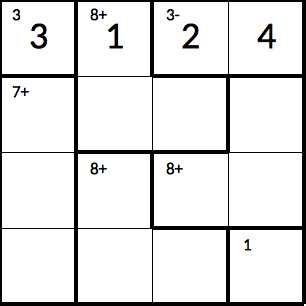
\includegraphics[scale=0.333]{Gambar/backtracking/State11}
\caption[\textit{State} 11]{\textit{State} 11}
\label{fig:analisisbt3}
\end{figure}

\item Karena semua kemungkinan angka untuk baris ke-1 dan kolom ke-4 telah dicoba dan gagal, maka algoritma harus mundur kembali ke (\textit{state} 7). Algoritma mencoba kemungkinan angka berikutnya, yaitu angka 3  (\textit{state} 12), seperti dapat dilihat pada Gambar~\ref{fig:analisisbt4}, tetapi angka 3 sudah pernah digunakan dalam baris tersebut. Algoritma lalu maju ke sel berikutnya.

\begin{figure}
\centering
\captionsetup{justification=centering}
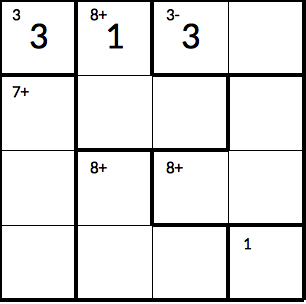
\includegraphics[scale=0.333]{Gambar/backtracking/State12}
\caption[\textit{State} 12]{\textit{State} 12}
\label{fig:analisisbt4}
\end{figure}

\item Algoritma lalu mencoba kemungkinan angka berikutnya, yaitu angka 4 (\textit{state} 13). Algoritma lalu maju ke sel berikutnya.
\item Algoritma lalu mengisikan sel pada baris ke-1 dan kolom ke-4 dengan angka 1 (\textit{state} 14), tetapi angka 1 sudah pernah digunakan dalam baris tersebut.
\item Algoritma lalu mencoba kemungkinan angka berikutnya, yaitu angka 2 (\textit{state} 15), tetapi hasilnya tidak sesuai dengan angka tujuan dari \textit{cage} tersebut.
\item Algoritma lalu mencoba kemungkinan angka berikutnya, yaitu angka 3 (\textit{state} 16), tetapi angka 3 sudah pernah digunakan dalam baris tersebut.
\item Algoritma lalu mencoba kemungkinan angka berikutnya, yaitu angka 4 (\textit{state} 17), seperti dapat dilihat pada Gambar~\ref{fig:analisisbt5}, tetapi angka 4 sudah pernah digunakan dalam baris tersebut.

\begin{figure}
\centering
\captionsetup{justification=centering}
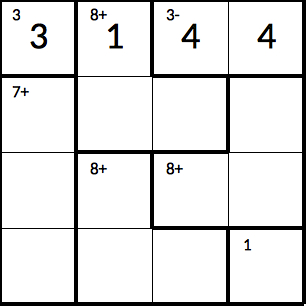
\includegraphics[scale=0.333]{Gambar/backtracking/State17}
\caption[\textit{State} 17]{\textit{State} 17}
\label{fig:analisisbt5}
\end{figure}

\item Karena semua kemungkinan angka untuk baris ke-1 dan kolom ke-3 dan ke-4 telah dicoba dan gagal, maka algoritma harus mundur kembali ke (\textit{state} 5). Algoritma mencoba kemungkinan angka berikutnya, yaitu angka 2  (\textit{state} 18), seperti dapat dilihat pada Gambar~\ref{fig:analisisbt6}. Algoritma lalu maju ke sel berikutnya.

\begin{figure}
\centering
\captionsetup{justification=centering}
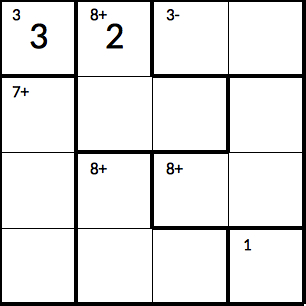
\includegraphics[scale=0.333]{Gambar/backtracking/State18}
\caption[\textit{State} 18]{\textit{State} 18}
\label{fig:analisisbt6}
\end{figure}

\item Algoritma lalu mengisikan sel pada baris ke-1 dan kolom ke-3 dengan angka 1 (\textit{state} 19), seperti dapat dilihat pada Gambar~\ref{fig:analisisbt7}. Algoritma lalu maju ke sel berikutnya.

\begin{figure}
\centering
\captionsetup{justification=centering}
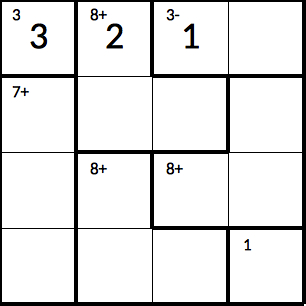
\includegraphics[scale=0.333]{Gambar/backtracking/State19}
\caption[\textit{State} 19]{\textit{State} 19}
\label{fig:analisisbt7}
\end{figure}

\item Algoritma lalu mengisikan sel pada baris ke-1 dan kolom ke-4 dengan angka 1 (\textit{state} 20), tetapi angka 1 sudah pernah digunakan dalam baris tersebut.
\item Algoritma lalu mencoba kemungkinan angka berikutnya, yaitu angka 2 (\textit{state} 21), tetapi angka 2 sudah pernah digunakan dalam baris tersebut.
\item Algoritma lalu mencoba kemungkinan angka berikutnya, yaitu angka 3 (\textit{state} 22), tetapi angka 3 sudah pernah digunakan dalam baris tersebut.
\item Algoritma lalu mencoba kemungkinan angka berikutnya, yaitu angka 4 (\textit{state} 23), dan ternyata hasilnya sesuai dengan angka tujuan dari \textit{cage} tersebut, seperti dapat dilihat pada Gambar~\ref{fig:analisisbt8}. Algoritma telah selesai mengisikan baris ke-1, sehingga bisa maju ke baris berikutnya.

\begin{figure}
\centering
\captionsetup{justification=centering}
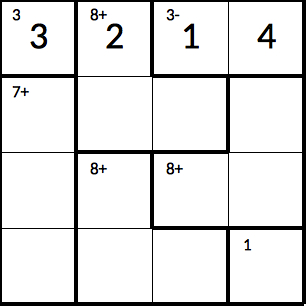
\includegraphics[scale=0.333]{Gambar/backtracking/State23}
\caption[\textit{State} 23]{\textit{State} 23}
\label{fig:analisisbt8}
\end{figure}

\item Algoritma lalu mengisikan sel pada baris ke-2 dan kolom ke-1 dengan angka 1 (\textit{state} 24), seperti dapat dilihat pada Gambar~\ref{fig:analisisbt9}. Algoritma lalu maju ke sel berikutnya.

\begin{figure}
\centering
\captionsetup{justification=centering}
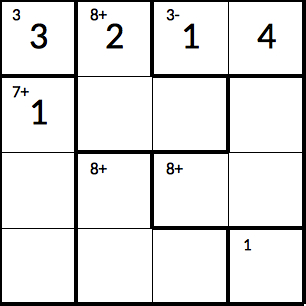
\includegraphics[scale=0.333]{Gambar/backtracking/State24}
\caption[\textit{State} 24]{\textit{State} 24}
\label{fig:analisisbt9}
\end{figure}

\item Algoritma lalu mengisikan sel pada baris ke-2 dan kolom ke-2 dengan angka 1 (\textit{state} 25), tetapi angka 1 sudah pernah digunakan dalam baris tersebut.
\item Algoritma lalu mencoba kemungkinan angka berikutnya, yaitu angka 2 (\textit{state} 26), tetapi angka 2 sudah pernah digunakan dalam kolom tersebut.
\item Algoritma lalu mencoba kemungkinan angka berikutnya, yaitu angka 3 (\textit{state} 27). Algoritma lalu maju ke sel berikutnya.
\item Algoritma lalu mengisikan sel pada baris ke-2 dan kolom ke-3 dengan angka 1 (\textit{state} 28), tetapi angka 1 sudah pernah digunakan dalam baris dan kolom tersebut.
\item Algoritma lalu mencoba kemungkinan angka berikutnya, yaitu angka 2 (\textit{state} 29), tetapi hasilnya tidak sesuai dengan angka tujuan dari \textit{cage} tersebut.
\item Algoritma lalu mencoba kemungkinan angka berikutnya, yaitu angka 3 (\textit{state} 30), tetapi angka 3 sudah pernah digunakan dalam baris tersebut.
\item Algoritma lalu mencoba kemungkinan angka berikutnya, yaitu angka 4 (\textit{state} 31), seperti dapat dilihat pada Gambar~\ref{fig:analisisbt10}, tetapi hasilnya tidak sesuai dengan angka tujuan dari \textit{cage} tersebut.

\begin{figure}
\centering
\captionsetup{justification=centering}
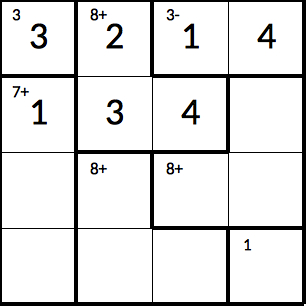
\includegraphics[scale=0.333]{Gambar/backtracking/State31}
\caption[\textit{State} 31]{\textit{State} 31}
\label{fig:analisisbt10}
\end{figure}

\item Karena semua kemungkinan angka untuk baris ke-2 dan kolom ke-3 telah dicoba dan gagal, maka algoritma harus mundur kembali ke (\textit{state} 27). Algoritma mencoba kemungkinan angka berikutnya, yaitu angka 4 (\textit{state} 32), seperti dapat dilihat pada Gambar~\ref{fig:analisisbt11}. Algoritma lalu maju ke sel berikutnya.

\begin{figure}
\centering
\captionsetup{justification=centering}
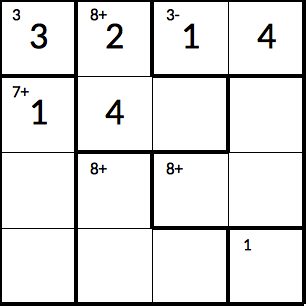
\includegraphics[scale=0.333]{Gambar/backtracking/State32}
\caption[\textit{State} 32]{\textit{State} 32}
\label{fig:analisisbt11}
\end{figure}

\item Algoritma lalu mengisikan sel pada baris ke-2 dan kolom ke-3 dengan angka 1 (\textit{state} 33), tetapi angka 1 sudah pernah digunakan dalam baris tersebut.
\item Algoritma lalu mencoba kemungkinan angka berikutnya, yaitu angka 2 (\textit{state} 34), dan ternyata hasilnya sesuai dengan angka tujuan dari \textit{cage} tersebut, seperti dapat dilihat pada Gambar~\ref{fig:analisisbt12}. Algoritma lalu maju ke sel berikutnya.

\begin{figure}
\centering
\captionsetup{justification=centering}
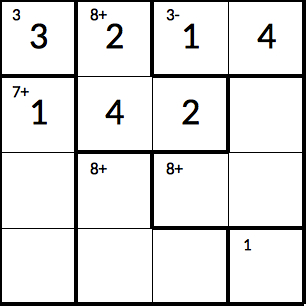
\includegraphics[scale=0.333]{Gambar/backtracking/State34}
\caption[\textit{State} 34]{\textit{State} 34}
\label{fig:analisisbt12}
\end{figure}

\item Algoritma lalu mengisikan sel pada baris ke-2 dan kolom ke-4 dengan angka 1 (\textit{state} 35), tetapi angka 1 sudah pernah digunakan dalam baris tersebut.
\item Algoritma lalu mencoba kemungkinan angka berikutnya, yaitu angka 2 (\textit{state} 36), tetapi angka 2 sudah pernah digunakan dalam baris tersebut.
\item Algoritma lalu mencoba kemungkinan angka berikutnya, yaitu angka 3 (\textit{state} 37), seperti dapat dilihat pada Gambar~\ref{fig:analisisbt13}. Algoritma telah selesai mengisikan baris ke-2, sehingga bisa maju ke baris berikutnya.

\begin{figure}
\centering
\captionsetup{justification=centering}
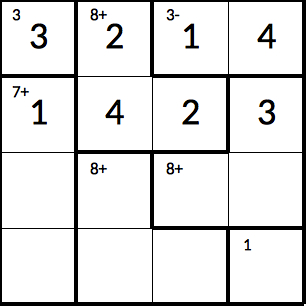
\includegraphics[scale=0.333]{Gambar/backtracking/State37}
\caption[\textit{State} 37]{\textit{State} 37}
\label{fig:analisisbt13}
\end{figure}

\item Algoritma lalu mengisikan sel pada baris ke-3 dan kolom ke-1 dengan angka 1 (\textit{state} 38), tetapi angka 1 sudah pernah digunakan dalam kolom tersebut.
\item Algoritma lalu mencoba kemungkinan angka berikutnya, yaitu angka 2 (\textit{state} 39). Algoritma lalu maju ke sel berikutnya.
\item Algoritma lalu mengisikan sel pada baris ke-3 dan kolom ke-2 dengan angka 1 (\textit{state} 40). Algoritma lalu maju ke sel berikutnya.
\item Algoritma lalu mengisikan sel pada baris ke-3 dan kolom ke-3 dengan angka 1 (\textit{state} 41), tetapi angka 1 sudah pernah digunakan dalam baris dan kolom tersebut.
\item Algoritma lalu mencoba kemungkinan angka berikutnya, yaitu angka 2 (\textit{state} 42), tetapi angka 2 sudah pernah digunakan dalam baris dan kolom tersebut.
\item Algoritma lalu mencoba kemungkinan angka berikutnya, yaitu angka 3 (\textit{state} 43). Algoritma lalu maju ke sel berikutnya.
\item Algoritma lalu mengisikan sel pada baris ke-3 dan kolom ke-4 dengan angka 1 (\textit{state} 44), tetapi angka 1 sudah pernah digunakan dalam baris tersebut.
\item Algoritma lalu mencoba kemungkinan angka berikutnya, yaitu angka 2 (\textit{state} 45), tetapi angka 2 sudah pernah digunakan dalam baris tersebut.
\item Algoritma lalu mencoba kemungkinan angka berikutnya, yaitu angka 3 (\textit{state} 46), tetapi angka 3 sudah pernah digunakan dalam baris dan kolom tersebut.
\item Algoritma lalu mencoba kemungkinan angka berikutnya, yaitu angka 4 (\textit{state} 47), seperti dapat dilihat pada Gambar~\ref{fig:analisisbt14}, tetapi hasilnya tidak sesuai dengan angka tujuan dari \textit{cage} tersebut.

\begin{figure}
\centering
\captionsetup{justification=centering}
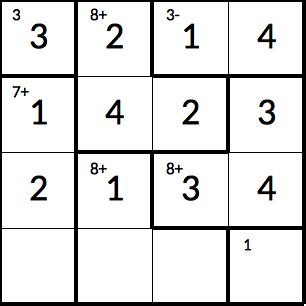
\includegraphics[scale=0.333]{Gambar/backtracking/State47}
\caption[\textit{State} 47]{\textit{State} 47}
\label{fig:analisisbt14}
\end{figure}

\item Karena semua kemungkinan angka untuk baris ke-3 dan kolom ke-4 telah dicoba dan gagal, maka algoritma harus mundur kembali ke (\textit{state} 43). Algoritma lalu mencoba kemungkinan angka berikutnya, yaitu angka 4 (\textit{state} 48), seperti dapat dilihat pada Gambar~\ref{fig:analisisbt15}. Algoritma lalu maju ke sel berikutnya.

\begin{figure}
\centering
\captionsetup{justification=centering}
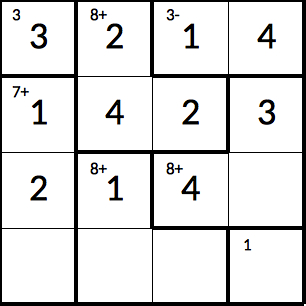
\includegraphics[scale=0.333]{Gambar/backtracking/State48}
\caption[\textit{State} 48]{\textit{State} 48}
\label{fig:analisisbt15}
\end{figure}

\item Algoritma lalu mengisikan sel pada baris ke-3 dan kolom ke-4 dengan angka 1 (\textit{state} 49), tetapi angka 1 sudah pernah digunakan dalam baris tersebut.
\item Algoritma lalu mencoba kemungkinan angka berikutnya, yaitu angka 2 (\textit{state} 50), tetapi angka 2 sudah pernah digunakan dalam baris tersebut.
\item Algoritma lalu mencoba kemungkinan angka berikutnya, yaitu angka 3 (\textit{state} 51), tetapi angka 3 sudah pernah digunakan dalam kolom tersebut.
\item Algoritma lalu mencoba kemungkinan angka berikutnya, yaitu angka 4 (\textit{state} 52), seperti dapat dilihat pada Gambar~\ref{fig:analisisbt16}, tetapi angka 3 sudah pernah digunakan dalam baris dan kolom tersebut.

\begin{figure}
\centering
\captionsetup{justification=centering}
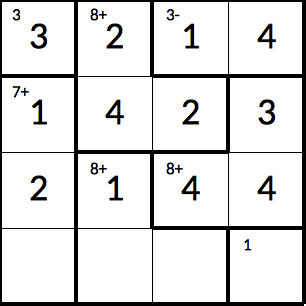
\includegraphics[scale=0.333]{Gambar/backtracking/State52}
\caption[\textit{State} 52]{\textit{State} 52}
\label{fig:analisisbt16}
\end{figure}

\item Karena semua kemungkinan angka untuk baris ke-3 dan kolom ke-4 telah dicoba dan gagal, maka algoritma harus mundur kembali ke (\textit{state} 48). Algoritma lalu mencoba kemungkinan angka berikutnya, yaitu angka 2 (\textit{state} 53) seperti dapat dilihat pada Gambar~\ref{fig:analisisbt17}, tetapi angka 2 sudah pernah digunakan dalam baris dan kolom tersebut.

\begin{figure}
\centering
\captionsetup{justification=centering}
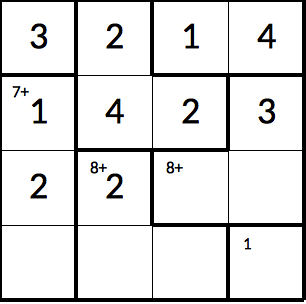
\includegraphics[scale=0.333]{Gambar/backtracking/State53}
\caption[\textit{State} 53]{\textit{State} 53}
\label{fig:analisisbt17}
\end{figure}

\item Algoritma lalu mencoba kemungkinan angka berikutnya, yaitu angka 3 (\textit{state} 54). Algoritma lalu maju ke sel berikutnya.
\item Algoritma lalu mengisikan sel pada baris ke-3 dan kolom ke-3 dengan angka 1 (\textit{state} 55), tetapi angka 1 sudah pernah digunakan dalam kolom tersebut.
\item Algoritma lalu mencoba kemungkinan angka berikutnya, yaitu angka 2 (\textit{state} 56), tetapi angka 2 sudah pernah digunakan dalam baris dan kolom tersebut.
\item Algoritma lalu mencoba kemungkinan angka berikutnya, yaitu angka 3 (\textit{state} 57), tetapi angka 3 sudah pernah digunakan dalam baris tersebut.
\item Algoritma lalu mencoba kemungkinan angka berikutnya, yaitu angka 4 (\textit{state} 58). Algoritma lalu maju ke sel berikutnya.
\item Algoritma lalu mengisikan sel pada baris ke-3 dan kolom ke-4 dengan angka 1 (\textit{state} 59). Algoritma telah selesai mengisikan baris ke-2, sehingga bisa maju ke baris berikutnya.
\item Algoritma lalu mengisikan sel pada baris ke-4 dan kolom ke-1 dengan angka 1 (\textit{state} 60), tetapi angka 1 sudah pernah digunakan dalam kolom tersebut.
\item Algoritma lalu mencoba kemungkinan angka berikutnya, yaitu angka 2 (\textit{state} 61), tetapi angka 2 sudah pernah digunakan dalam kolom tersebut.
\item Algoritma lalu mencoba kemungkinan angka berikutnya, yaitu angka 3 (\textit{state} 62), tetapi angka 3 sudah pernah digunakan dalam kolom tersebut.
\item Algoritma lalu mencoba kemungkinan angka berikutnya, yaitu angka 4 (\textit{state} 63). Algoritma lalu maju ke sel berikutnya.
\item Algoritma lalu mengisikan sel pada baris ke-4 dan kolom ke-2 dengan angka 1 (\textit{state} 64). Algoritma lalu maju ke sel berikutnya.
\item Algoritma lalu mengisikan sel pada baris ke-4 dan kolom ke-3 dengan angka 1 (\textit{state} 65), tetapi angka 1 sudah pernah digunakan dalam baris dan kolom tersebut.
\item Algoritma lalu mencoba kemungkinan angka berikutnya, yaitu angka 2 (\textit{state} 66), tetapi angka 2 sudah pernah digunakan dalam kolom tersebut.
\item Algoritma lalu mencoba kemungkinan angka berikutnya, yaitu angka 3 (\textit{state} 67), tetapi hasilnya tidak sesuai dengan angka tujuan dari \textit{cage} tersebut.
\item Algoritma lalu mencoba kemungkinan angka berikutnya, yaitu angka 4 (\textit{state} 68), seperti dapat dilihat di Gambar~\ref{fig:analisisbt18}. tetapi angka 4 sudah pernah digunakan dalam baris dan kolom tersebut.

\begin{figure}
\centering
\captionsetup{justification=centering}
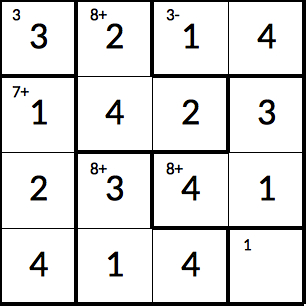
\includegraphics[scale=0.333]{Gambar/backtracking/State68}
\caption[\textit{State} 68]{\textit{State} 68}
\label{fig:analisisbt18}
\end{figure}

\item Karena semua kemungkinan angka untuk baris ke-4 dan kolom ke-3 telah dicoba dan gagal, maka algoritma harus mundur kembali ke (\textit{state} 64). Algoritma lalu mencoba kemungkinan angka berikutnya, yaitu angka 2 (\textit{state} 69), seperti dapat dilihat pada Gambar~\ref{fig:analisisbt19}, tetapi angka 2 sudah pernah digunakan dalam kolom tersebut.

\begin{figure}
\centering
\captionsetup{justification=centering}
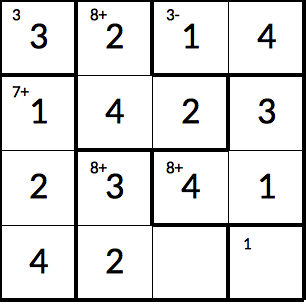
\includegraphics[scale=0.333]{Gambar/backtracking/State69}
\caption[\textit{State} 69]{\textit{State} 69}
\label{fig:analisisbt19}
\end{figure}

\item Algoritma lalu mencoba kemungkinan angka berikutnya, yaitu angka 3 (\textit{state} 70), tetapi angka 3 sudah pernah digunakan dalam kolom tersebut.
\item Algoritma lalu mencoba kemungkinan angka berikutnya, yaitu angka 4 (\textit{state} 71), seperti dapat dilihat di Gambar~\ref{fig:analisisbt20}, tetapi angka 4 sudah pernah digunakan dalam kolom tersebut.

\begin{figure}
\centering
\captionsetup{justification=centering}
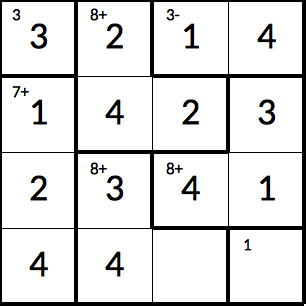
\includegraphics[scale=0.333]{Gambar/backtracking/State71}
\caption[\textit{State} 71]{\textit{State} 71}
\label{fig:analisisbt20}
\end{figure}

\item Karena semua kemungkinan angka untuk baris ke-4 dan kolom ke-1 dan ke-2 telah dicoba dan gagal, maka algoritma harus mundur kembali ke (\textit{state} 59). Algoritma lalu mencoba kemungkinan angka berikutnya, yaitu angka 2 (\textit{state} 72), seperti dapat dilihat pada Gambar~\ref{fig:analisisbt21}, tetapi angka 2 sudah pernah digunakan dalam baris tersebut.

\begin{figure}
\centering
\captionsetup{justification=centering}
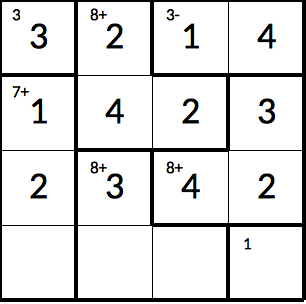
\includegraphics[scale=0.333]{Gambar/backtracking/State72}
\caption[\textit{State} 72]{\textit{State} 72}
\label{fig:analisisbt21}
\end{figure}

\item Algoritma lalu mencoba kemungkinan angka berikutnya, yaitu angka 3 (\textit{state} 73), tetapi angka 3 sudah pernah digunakan dalam baris dan kolom tersebut.
\item Algoritma lalu mencoba kemungkinan angka berikutnya, yaitu angka 4 (\textit{state} 74), seperti dapat dilihat di Gambar~\ref{fig:analisisbt22}, tetapi angka 4 sudah pernah digunakan dalam baris dan kolom tersebut.

\begin{figure}
\centering
\captionsetup{justification=centering}
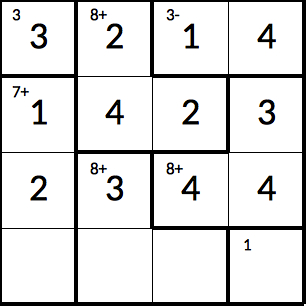
\includegraphics[scale=0.333]{Gambar/backtracking/State74}
\caption[\textit{State} 74]{\textit{State} 74}
\label{fig:analisisbt22}
\end{figure}

\item Karena semua kemungkinan angka untuk baris ke-3 dan kolom ke-3 dan ke-4 telah dicoba dan gagal, maka algoritma harus mundur kembali ke (\textit{state} 54). Algoritma lalu mencoba kemungkinan angka berikutnya, yaitu angka 4 (\textit{state} 75), seperti dapat dilihat pada Gambar~\ref{fig:analisisbt23}, tetapi angka 4 sudah pernah digunakan dalam kolom tersebut.

\begin{figure}
\centering
\captionsetup{justification=centering}
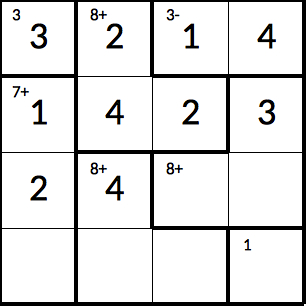
\includegraphics[scale=0.333]{Gambar/backtracking/State75}
\caption[\textit{State} 75]{\textit{State} 75}
\label{fig:analisisbt23}
\end{figure}

\item Karena semua kemungkinan angka untuk baris ke-3 dan kolom ke-2 telah dicoba dan gagal, maka algoritma harus mundur kembali ke (\textit{state} 54). Algoritma lalu mencoba kemungkinan angka berikutnya, yaitu angka 3 (\textit{state} 76), seperti dapat dilihat pada Gambar~\ref{fig:analisisbt24}, tetapi angka 3 sudah pernah digunakan dalam kolom tersebut.

\begin{figure}
\centering
\captionsetup{justification=centering}
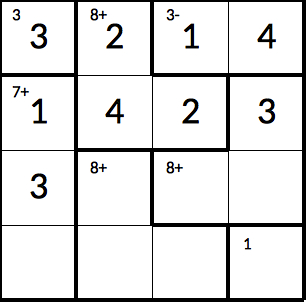
\includegraphics[scale=0.333]{Gambar/backtracking/State76}
\caption[\textit{State} 76]{\textit{State} 76}
\label{fig:analisisbt24}
\end{figure}

\item Algoritma lalu mencoba kemungkinan angka berikutnya, yaitu angka 4 (\textit{state} 77), seperti dapat dilihat di Gambar~\ref{fig:analisisbt25}. Algoritma lalu maju ke sel berikutnya.

\begin{figure}
\centering
\captionsetup{justification=centering}
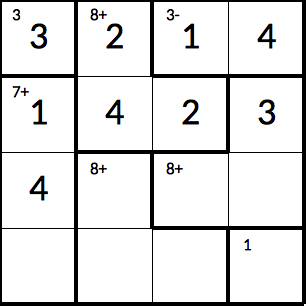
\includegraphics[scale=0.333]{Gambar/backtracking/State77}
\caption[\textit{State} 77]{\textit{State} 77}
\label{fig:analisisbt25}
\end{figure}

\item Algoritma lalu mengisikan sel pada baris ke-3 dan kolom ke-2 dengan angka 1 (\textit{state} 78), seperti dapat dilihat di Gambar~\ref{fig:analisisbt26}. Algoritma lalu maju ke sel berikutnya.

\begin{figure}
\centering
\captionsetup{justification=centering}
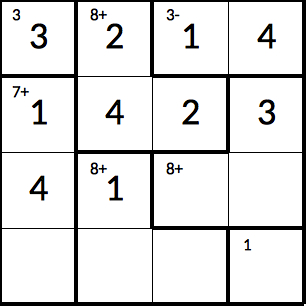
\includegraphics[scale=0.333]{Gambar/backtracking/State78}
\caption[\textit{State} 78]{\textit{State} 78}
\label{fig:analisisbt26}
\end{figure}

\item Algoritma lalu mengisikan sel pada baris ke-3 dan kolom ke-3 dengan angka 1 (\textit{state} 79), tetapi angka 1 sudah pernah digunakan dalam baris dan kolom tersebut.
\item Algoritma lalu mencoba kemungkinan angka berikutnya, yaitu angka 2 (\textit{state} 80), tetapi angka 2 sudah pernah digunakan dalam kolom tersebut.
\item Algoritma lalu mencoba kemungkinan angka berikutnya, yaitu angka 3 (\textit{state} 81), seperti dapat dilihat pada Gambar~\ref{fig:analisisbt27}. Algoritma lalu maju ke sel berikutnya.

\begin{figure}
\centering
\captionsetup{justification=centering}
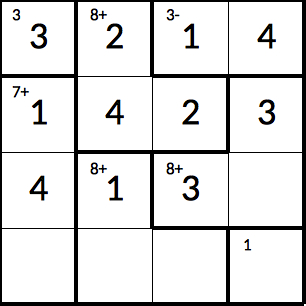
\includegraphics[scale=0.333]{Gambar/backtracking/State81}
\caption[\textit{State} 81]{\textit{State} 81}
\label{fig:analisisbt27}
\end{figure}

\item Algoritma lalu mengisikan sel pada baris ke-3 dan kolom ke-3 dengan angka 1 (\textit{state} 82), tetapi angka 1 sudah pernah digunakan dalam baris tersebut.
\item Algoritma lalu mencoba kemungkinan angka berikutnya, yaitu angka 2 (\textit{state} 83), dan ternyata hasilnya sesuai dengan angka tujuan dari \textit{cage} tersebut, seperti dapat dilihat pada Gambar~\ref{fig:analisisbt28}. Algoritma telah selesai mengisikan baris ke-3, sehingga bisa maju ke baris berikutnya.

\begin{figure}
\centering
\captionsetup{justification=centering}
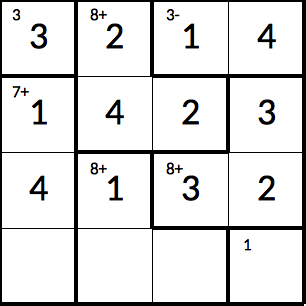
\includegraphics[scale=0.333]{Gambar/backtracking/State83}
\caption[\textit{State} 83]{\textit{State} 83}
\label{fig:analisisbt28}
\end{figure}

\item Algoritma lalu mengisikan sel pada baris ke-4 dan kolom ke-1 dengan angka 1 (\textit{state} 84), tetapi angka 1 sudah pernah digunakan dalam kolom tersebut.
\item Algoritma lalu mencoba kemungkinan angka berikutnya, yaitu angka 2 (\textit{state} 85), dan ternyata hasilnya sesuai dengan angka tujuan dari \textit{cage} tersebut, seperti dapat dilihat pada Gambar~\ref{fig:analisisbt29}. Algoritma lalu maju ke sel berikutnya.

\begin{figure}
\centering
\captionsetup{justification=centering}
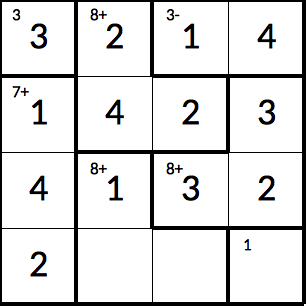
\includegraphics[scale=0.333]{Gambar/backtracking/State85}
\caption[\textit{State} 85]{\textit{State} 85}
\label{fig:analisisbt29}
\end{figure}

\item Algoritma lalu mengisikan sel pada baris ke-4 dan kolom ke-2 dengan angka 1 (\textit{state} 86), tetapi angka 1 sudah pernah digunakan dalam kolom tersebut.
\item Algoritma lalu mencoba kemungkinan angka berikutnya, yaitu angka 2 (\textit{state} 87), tetapi angka 2 sudah pernah digunakan dalam baris dan kolom tersebut.
\item Algoritma lalu mencoba kemungkinan angka berikutnya, yaitu angka 3 (\textit{state} 88), seperti dapat dilihat pada Gambar~\ref{fig:analisisbt30}. Algoritma lalu maju ke sel berikutnya.

\begin{figure}
\centering
\captionsetup{justification=centering}
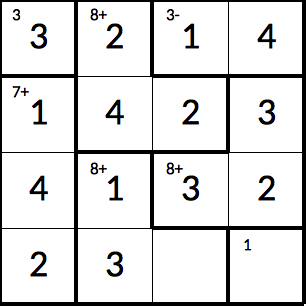
\includegraphics[scale=0.333]{Gambar/backtracking/State88}
\caption[\textit{State} 88]{\textit{State} 88}
\label{fig:analisisbt30}
\end{figure}

\item Algoritma lalu mengisikan sel pada baris ke-4 dan kolom ke-3 dengan angka 1 (\textit{state} 89), tetapi angka 1 sudah pernah digunakan dalam baris dan kolom tersebut.
\item Algoritma lalu mencoba kemungkinan angka berikutnya, yaitu angka 2 (\textit{state} 90), tetapi angka 2 sudah pernah digunakan dalam baris dan kolom tersebut.
\item Algoritma lalu mencoba kemungkinan angka berikutnya, yaitu angka 3 (\textit{state} 91), tetapi angka 3 sudah pernah digunakan dalam kolom tersebut.
\item Algoritma lalu mencoba kemungkinan angka berikutnya, yaitu angka 4 (\textit{state} 92), dan ternyata hasilnya sesuai dengan angka tujuan dari \textit{cage} tersebut, seperti dapat dilihat pada Gambar~\ref{fig:analisisbt31}. Algoritma lalu maju ke sel berikutnya.

\begin{figure}
\centering
\captionsetup{justification=centering}
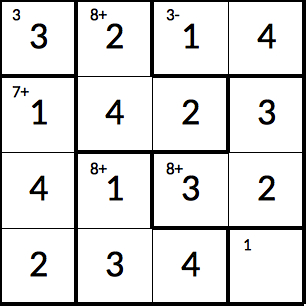
\includegraphics[scale=0.333]{Gambar/backtracking/State92}
\caption[\textit{State} 92]{\textit{State} 92}
\label{fig:analisisbt31}
\end{figure}

\item Algoritma lalu mengisikan sel pada baris ke-4 dan kolom ke-4 dengan angka 1 (\textit{state} 93), dan ternyata hasilnya sesuai dengan angka tujuan dari \textit{cage} tersebut, seperti dapat dilihat pada Gambar~\ref{fig:analisisbt32}. Algoritma \textit{backtracking} telah selesai mengisi semua sel dalam permainan teka-teki Calcudoku ini dengan benar.

\begin{figure}
\centering
\captionsetup{justification=centering}
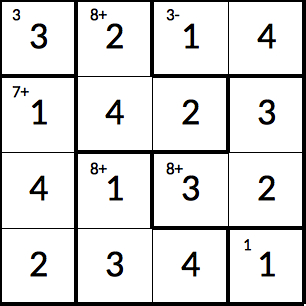
\includegraphics[scale=0.333]{Gambar/backtracking/State93}
\caption[\textit{State} 93]{\textit{State} 93}
\label{fig:analisisbt32}
\end{figure}

\end{itemize}

Algoritma ini mencapai solusinya pada state 93, seperti pada \textit{state space tree} yang digambarkan dalam Gambar~\ref{fig:analisisbt33}. \textit{State space tree} ini telah mencapai simpul tujuannya, yaitu simpul 93, dengan jalur 3-2-1-4-1-4-2-3-4-1-3-2-2-3-4-1.

\begin{landscape}
\begin{figure}
\centering
\captionsetup{justification=centering}
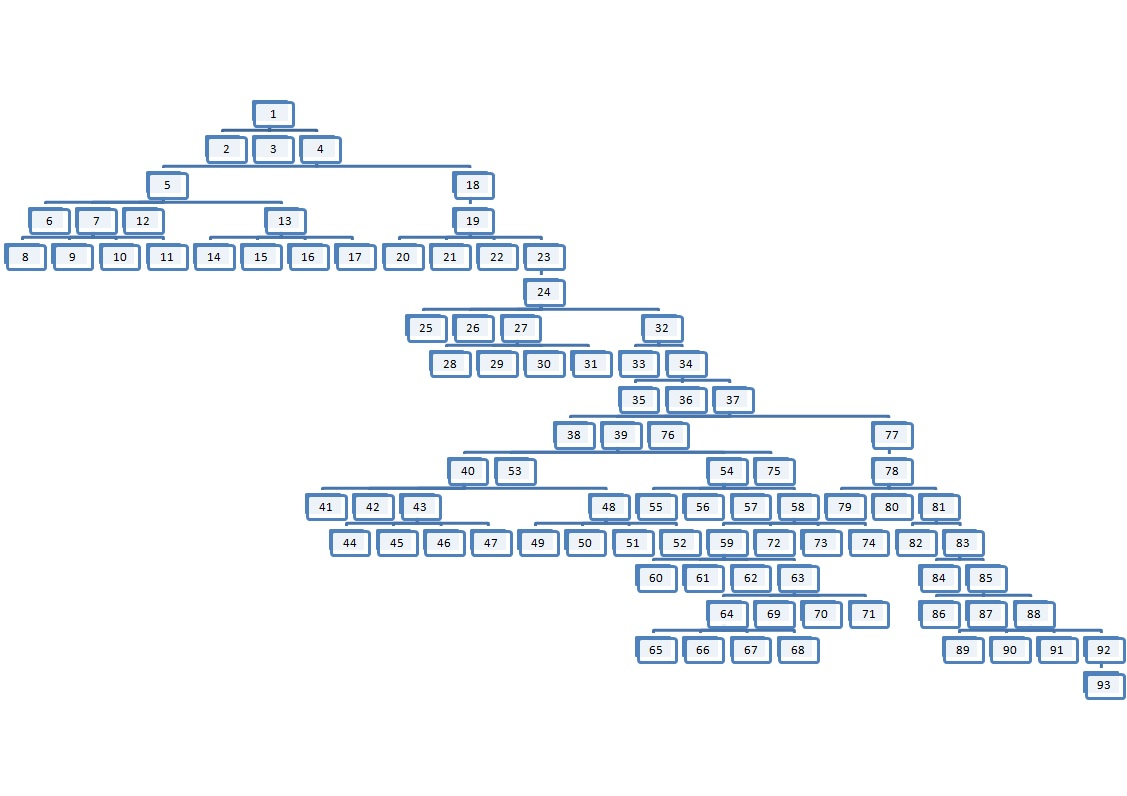
\includegraphics[scale=0.75]{Gambar/backtracking/StateSpaceTree}
\caption[\textit{State space tree} yang dikembangkan dalam proses menyelesaikan teka-teki Calcudoku yang digambarkan pada Gambar~\ref{fig:analisisbt1}]{\textit{State space tree} yang dikembangkan dalam proses menyelesaikan teka-teki Calcudoku yang digambarkan pada Gambar~\ref{fig:analisisbt1}}
\label{fig:analisisbt33}
\end{figure}
\end{landscape}

\textbf{Algoritma \textit{Hybrid Genetic}}

Untuk mengilustrasikan cara kerja algoritma \textit{hybrid genetic}, akan digunakan permainan teka-teki Calcudoku yang digambarkan pada Gambar~\ref{fig:analisishg1} sebagai contoh. Algoritma \textit{hybrid genetic} dimulai dengan mencoba menyelesaikan permainan teka-teki Calcudoku dengan algoritma \textit{rule based}.

\begin{figure}
\centering
\captionsetup{justification=centering}
\includegraphics[scale=0.333]{Gambar/hybridgenetic/Puzzle}
\caption[Contoh permainan teka-teki Calcudoku dengan ukuran \textit{grid} 6 x 6 yang belum diselesaikan, seperti yang digambarkan pada Gambar~\ref{fig:hybrid1}. \cite{JohannaLukasSaputra}]{Contoh permainan teka-teki Calcudoku dengan ukuran \textit{grid} 6 x 6 yang belum diselesaikan, seperti yang digambarkan pada Gambar~\ref{fig:hybrid1}. \cite{JohannaLukasSaputra}}
\label{fig:analisishg1}
\end{figure}

\textbf{Algoritma \textit{Rule Based}}

Sel pada baris ke-4 dan kolom ke-6 adalah bagian dari sebuah \textit{cage} yang berukuran hanya 1 sel, dan oleh karena itu, angka tujuan dari sel tersebut adalah angka tujuan dari \textit{cage} tersebut (aturan \textit{single square}). Angka tujuan dari \textit{cage} tersebut adalah 1, dan oleh karena itu sel tersebut dapat langsung diisi dengan angka 1, seperti dapat dilihat pada Gambar~\ref{fig:analisishg2}.

Sayangnya, algoritma \textit{rule based} gagal dalam mengisi sel-sel lainnya berdasarkan aturan-aturan yang telah didefinisikan setelah beberapa kali percobaan, sehingga algoritma \textit{hybrid genetic} akan mencoba menyelesaikan teka-teki Calcudoku dengan algoritma genetik.

\begin{figure}
\centering
\captionsetup{justification=centering}
\includegraphics[scale=0.333]{Gambar/hybridgenetic/PuzzleAfterRuleBased}
\caption[Permainan teka-teki Calcudoku setelah diselesaikan dengan algoritma \textit{rule based}]{Permainan teka-teki Calcudoku setelah diselesaikan dengan algoritma \textit{rule based}}
\label{fig:analisishg2}
\end{figure}

\textbf{Algoritma Genetik}

Dalam contoh ini, parameter-parameter untuk algoritma genetik yang akan digunakan untuk teka-teki Calcudoku ini ditunjukkan pada Tabel~\ref{tab:analisishg1}. Setiap generasi terdiri dari 12 kromosom. \begin{math}40\% \times 12 \approx 5\end{math} kromosom diambil dari generasi sebelumnya (\textit{elitism}). \begin{math}50\% \times 12 \approx 6\end{math} kromosom adalah hasil dari pembentukan kromosom-kromosom baru dengan operasi kawin silang, dan \begin{math}10\% \times 12 \approx 1\end{math} kromosom adalah hasil dari pembentukan kromosom-kromosom baru dengan operasi mutasi. Biasanya, operasi kawin silang akan menghasilkan 2 kromosom baru, tetapi dalam kasus ini ditentukan bahwa operasi kawin silang hanya akan menghasilkan 1 kromosom baru. Untuk mengilustrasikan cara kerja algoritma genetik, hanya 3 generasi pertama yang akan dibahas.

Setiap sel mempunyai nilai kelayakan. Nilai kelayakan dari sebuah sel akan bernilai 1 jika nilai dari semua sel yang merupakan bagian dari \textit{cage} yang salah satu selnya adalah sel tersebut menghasilkan nilai tujuan setelah dihitung menggunakan operator yang telah ditentukan dan tidak ada pengulangan angka di dalam baris tersebut maupun kolom tersebut, dan bernilai 0 jika nilai dari semua sel yang merupakan bagian dari \textit{cage} yang salah satu selnya adalah sel tersebut tidak menghasilkan nilai tujuan setelah dihitung menggunakan operator yang telah ditentukan atau ada pengulangan angka di dalam baris tersebut maupun kolom tersebut. Nilai kelayakan sel untuk setiap sel dalam sebuah baris dijumlahkan, lalu dibagi dengan jumlah kolom dalam baris tersebut, dan hasilnya adalah nilai kelayakan baris. Nilai kelayakan baris untuk setiap baris dalam sebuah teka-teki dijumlahkan, lalu dibagi dengan jumlah baris dalam teka-teki tersebut, dan hasilnya adalah nilai kelayakan teka-teki.

\begin{table}
\centering
\captionsetup{justification=centering}
\begin{tabular}{| l | l |}
\hline
Parameter & Nilai \\
\hline \hline
Ukuran Populasi & 12 \\
\hline
Probabilitas \textit{Elitism} & 40\% \\
\hline
Probabilitas silang & 50\% \\
\hline
Probabilitas Mutasi & 10\% \\
\hline
\end{tabular}
\caption[Tabel parameter untuk algoritma genetik yang akan digunakan untuk menyelesaikan teka-teki Calcudoku yang digambarkan pada Gambar~\ref{fig:analisishg2}]{Tabel parameter untuk algoritma genetik yang akan digunakan untuk menyelesaikan teka-teki Calcudoku yang digambarkan pada Gambar~\ref{fig:analisishg2}}
\label{tab:analisishg1}
\end{table}

Algoritma genetik dimulai dengan membangkitkan kromosom-kromosom baru sebanyak ukuran populasi yang telah ditentukan. Dalam contoh ini, ukuran populasi adalah 12, maka algoritma akan membangkitkan 12 kromosom baru. Ke-12 kromosom awal ini adalah bagian dari generasi pertama. Gambar~\ref{fig:analisisg1k1} menggambarkan Kromosom 1, gambar~\ref{fig:analisisg1k2} menggambarkan Kromosom 2, gambar~\ref{fig:analisisg1k3} menggambarkan Kromosom 3, gambar~\ref{fig:analisisg1k4} menggambarkan Kromosom 4, gambar~\ref{fig:analisisg1k5} menggambarkan Kromosom 5, gambar~\ref{fig:analisisg1k6} menggambarkan Kromosom 6, gambar~\ref{fig:analisisg1k7} menggambarkan Kromosom 7, gambar~\ref{fig:analisisg1k8} menggambarkan Kromosom 8, gambar~\ref{fig:analisisg1k9} menggambarkan Kromosom 9, gambar~\ref{fig:analisisg1k10} menggambarkan Kromosom 10, gambar~\ref{fig:analisisg1k11} menggambarkan Kromosom 11, dan gambar~\ref{fig:analisisg1k12} menggambarkan Kromosom 12.

\clearpage

\begin{figure}
\centering
\captionsetup{justification=centering}
\includegraphics[scale=0.333]{Gambar/hybridgenetic/Generation1Chromosome1}
\caption[Kromosom 1 dalam Generasi ke-1]{Kromosom 1 dalam Generasi ke-1}
\label{fig:analisisg1k1}
\end{figure}

\begin{figure}
\centering
\captionsetup{justification=centering}
\includegraphics[scale=0.333]{Gambar/hybridgenetic/Generation1Chromosome2}
\caption[Kromosom 2 dalam Generasi ke-1]{Kromosom 2 dalam Generasi ke-1}
\label{fig:analisisg1k2}
\end{figure}

\begin{figure}
\centering
\captionsetup{justification=centering}
\includegraphics[scale=0.333]{Gambar/hybridgenetic/Generation1Chromosome3}
\caption[Kromosom 3 dalam Generasi ke-1]{Kromosom 3 dalam Generasi ke-1}
\label{fig:analisisg1k3}
\end{figure}

\begin{figure}
\centering
\captionsetup{justification=centering}
\includegraphics[scale=0.333]{Gambar/hybridgenetic/Generation1Chromosome4}
\caption[Kromosom 4 dalam Generasi ke-1]{Kromosom 4 dalam Generasi ke-1}
\label{fig:analisisg1k4}
\end{figure}

\begin{figure}
\centering
\captionsetup{justification=centering}
\includegraphics[scale=0.333]{Gambar/hybridgenetic/Generation1Chromosome5}
\caption[Kromosom 5 dalam Generasi ke-1]{Kromosom 5 dalam Generasi ke-1}
\label{fig:analisisg1k5}
\end{figure}

\begin{figure}
\centering
\captionsetup{justification=centering}
\includegraphics[scale=0.333]{Gambar/hybridgenetic/Generation1Chromosome6}
\caption[Kromosom 6 dalam Generasi ke-1]{Kromosom 6 dalam Generasi ke-1}
\label{fig:analisisg1k6}
\end{figure}

\begin{figure}
\centering
\captionsetup{justification=centering}
\includegraphics[scale=0.333]{Gambar/hybridgenetic/Generation1Chromosome7}
\caption[Kromosom 7 dalam Generasi ke-1]{Kromosom 7 dalam Generasi ke-1}
\label{fig:analisisg1k7}
\end{figure}

\begin{figure}
\centering
\captionsetup{justification=centering}
\includegraphics[scale=0.333]{Gambar/hybridgenetic/Generation1Chromosome8}
\caption[Kromosom 8 dalam Generasi ke-1]{Kromosom 8 dalam Generasi ke-1}
\label{fig:analisisg1k8}
\end{figure}

\begin{figure}
\centering
\captionsetup{justification=centering}
\includegraphics[scale=0.333]{Gambar/hybridgenetic/Generation1Chromosome9}
\caption[Kromosom 9 dalam Generasi ke-1]{Kromosom 9 dalam Generasi ke-1}
\label{fig:analisisg1k9}
\end{figure}

\begin{figure}
\centering
\captionsetup{justification=centering}
\includegraphics[scale=0.333]{Gambar/hybridgenetic/Generation1Chromosome10}
\caption[Kromosom 10 dalam Generasi ke-1]{Kromosom 10 dalam Generasi ke-1}
\label{fig:analisisg1k10}
\end{figure}

\begin{figure}
\centering
\captionsetup{justification=centering}
\includegraphics[scale=0.333]{Gambar/hybridgenetic/Generation1Chromosome11}
\caption[Kromosom 11 dalam Generasi ke-1]{Kromosom 11 dalam Generasi ke-1}
\label{fig:analisisg1k11}
\end{figure}

\begin{figure}
\centering
\captionsetup{justification=centering}
\includegraphics[scale=0.333]{Gambar/hybridgenetic/Generation1Chromosome12}
\caption[Kromosom 12 dalam Generasi ke-1]{Kromosom 12 dalam Generasi ke-1}
\label{fig:analisisg1k12}
\end{figure}

\clearpage

Berdasarkan nilai kelayakan untuk kromosom-kromosom pada Generasi ke-1 yang ditampilkan pada Tabel~\ref{tab:analisishg2}, 5 kromosom terbaik akan diambil untuk menjadi bagian dari Generasi ke-2. Ke-5 kromosom yang terpilih adalah Kromosom 12, Kromosom 5, Kromosom 7, Kromosom 11, dan Kromosom 1.

\begin{table}
\centering
\captionsetup{justification=centering}
\begin{tabular}{| l | l |}
\hline
Nomor Kromosom & Nilai Kelayakan \\
\hline \hline
1 & 0,3333 \\
\hline
2 & 0,3056 \\
\hline
3 & 0,25 \\
\hline
4 & 0,2222 \\
\hline
5 & 0,4444 \\
\hline
6 & 0,1389 \\
\hline
7 & 0,3889 \\
\hline
8 & 0,25 \\
\hline
9 & 0,1389 \\
\hline
10 & 0,3056 \\
\hline
11 & 0,3889 \\
\hline
12 & 0,5556 \\
\hline
\end{tabular}
\caption[Tabel nilai kelayakan untuk kromosom-kromsom pada Generasi ke-1]{Tabel nilai kelayakan untuk kromosom-kromsom pada Generasi ke-1}
\label{tab:analisishg2}
\end{table}

Untuk Generasi ke-2, 5 kromosom adalah 5 kromosom terbaik dari Generasi ke-1, 6 kromosom adalah hasil kawin silang dari 2 kromosom dari Generasi ke-1, dan 1 kromosom adalah hasil mutasi dari 1 kromosom dari Generasi ke-1.

Gambar~\ref{fig:analisisg2k1} menggambarkan Kromosom 1, yaitu Kromosom 12 dari Generasi ke-1, gambar~\ref{fig:analisisg2k2} menggambarkan Kromosom 2, yaitu Kromosom 5 dari Generasi ke-1, gambar~\ref{fig:analisisg2k3} menggambarkan Kromosom 3, yaitu Kromosom 7 dari Generasi ke-1, gambar~\ref{fig:analisisg2k4} menggambarkan Kromosom 4, yaitu Kromosom 11 dari Generasi ke-1, gambar~\ref{fig:analisisg2k5} menggambarkan Kromosom 5, yaitu Kromosom 1 dari Generasi ke-1, gambar~\ref{fig:analisisg2k6} menggambarkan Kromosom 6, yayaitu hasil kawin silang dari Kromosom 5 dan Kromosom 12 dari Generasi ke-1, gambar~\ref{fig:analisisg2k7} menggambarkan Kromosom 7, yayaitu hasil kawin silang dari Kromosom 7 dan Kromosom 11 dari Generasi ke-1, gambar~\ref{fig:analisisg2k8} menggambarkan Kromosom 8, yaitu hasil Kawin Sialng dari Kromosom 2 dan Kromosom 10 dari Generasi ke-1, gambar~\ref{fig:analisisg2k9} menggambarkan Kromosom 9, yaitu hasil kawin silang dari Kromosom 6 dan Kromosom 9 dari Generasi ke-1, gambar~\ref{fig:analisisg2k10} menggambarkan Kromosom 10, yaitu hasil kawin silang dari Kromosom 7 dan Kromosom 12 dari Generasi ke-1, gambar~\ref{fig:analisisg2k11} menggambarkan Kromosom 11, yaitu hasil kawin silang dari Kromosom 11 dan Kromosom 12 dari Generasi ke-1, dan gambar~\ref{fig:analisisg2k12} menggambarkan Kromosom 12, yaitu hasil mutasi dari Kromosom 12 dari Generasi ke-1.

\clearpage

\begin{figure}
\centering
\captionsetup{justification=centering}
\includegraphics[scale=0.333]{Gambar/hybridgenetic/Generation2Chromosome1}
\caption[Kromosom 1 dalam Generasi ke-2]{Kromosom 1 dalam Generasi ke-2}
\label{fig:analisisg2k1}
\end{figure}

\begin{figure}
\centering
\captionsetup{justification=centering}
\includegraphics[scale=0.333]{Gambar/hybridgenetic/Generation2Chromosome2}
\caption[Kromosom 2 dalam Generasi ke-2]{Kromosom 2 dalam Generasi ke-2}
\label{fig:analisisg2k2}
\end{figure}

\begin{figure}
\centering
\captionsetup{justification=centering}
\includegraphics[scale=0.333]{Gambar/hybridgenetic/Generation2Chromosome3}
\caption[Kromosom 3 dalam Generasi ke-2]{Kromosom 3 dalam Generasi ke-2}
\label{fig:analisisg2k3}
\end{figure}

\begin{figure}
\centering
\captionsetup{justification=centering}
\includegraphics[scale=0.333]{Gambar/hybridgenetic/Generation2Chromosome4}
\caption[Kromosom 4 dalam Generasi ke-2]{Kromosom 4 dalam Generasi ke-2}
\label{fig:analisisg2k4}
\end{figure}

\begin{figure}
\centering
\captionsetup{justification=centering}
\includegraphics[scale=0.333]{Gambar/hybridgenetic/Generation2Chromosome5}
\caption[Kromosom 5 dalam Generasi ke-2]{Kromosom 5 dalam Generasi ke-2}
\label{fig:analisisg2k5}
\end{figure}

\begin{figure}
\centering
\captionsetup{justification=centering}
\includegraphics[scale=0.333]{Gambar/hybridgenetic/Generation2Chromosome6}
\caption[Kromosom 6 dalam Generasi ke-2]{Kromosom 6 dalam Generasi ke-2}
\label{fig:analisisg2k6}
\end{figure}

\begin{figure}
\centering
\captionsetup{justification=centering}
\includegraphics[scale=0.333]{Gambar/hybridgenetic/Generation2Chromosome7}
\caption[Kromosom 7 dalam Generasi ke-2]{Kromosom 7 dalam Generasi ke-2}
\label{fig:analisisg2k7}
\end{figure}

\begin{figure}
\centering
\captionsetup{justification=centering}
\includegraphics[scale=0.333]{Gambar/hybridgenetic/Generation2Chromosome8}
\caption[Kromosom 8 dalam Generasi ke-2]{Kromosom 8 dalam Generasi ke-2}
\label{fig:analisisg2k8}
\end{figure}

\begin{figure}
\centering
\captionsetup{justification=centering}
\includegraphics[scale=0.333]{Gambar/hybridgenetic/Generation2Chromosome9}
\caption[Kromosom 9 dalam Generasi ke-2]{Kromosom 9 dalam Generasi ke-2}
\label{fig:analisisg2k9}
\end{figure}

\begin{figure}
\centering
\captionsetup{justification=centering}
\includegraphics[scale=0.333]{Gambar/hybridgenetic/Generation2Chromosome10}
\caption[Kromosom 10 dalam Generasi ke-2]{Kromosom 10 dalam Generasi ke-2}
\label{fig:analisisg2k10}
\end{figure}

\begin{figure}
\centering
\captionsetup{justification=centering}
\includegraphics[scale=0.333]{Gambar/hybridgenetic/Generation2Chromosome11}
\caption[Kromosom 11 dalam Generasi ke-2]{Kromosom 11 dalam Generasi ke-2}
\label{fig:analisisg2k11}
\end{figure}

\begin{figure}
\centering
\captionsetup{justification=centering}
\includegraphics[scale=0.333]{Gambar/hybridgenetic/Generation2Chromosome12}
\caption[Kromosom 12 dalam Generasi ke-2]{Kromosom 12 dalam Generasi ke-2}
\label{fig:analisisg2k12}
\end{figure}

\clearpage

Berdasarkan nilai kelayakan untuk kromosom-kromosom pada Generasi ke-2 yang ditampilkan pada Tabel~\ref{tab:analisishg3}, 5 kromosom terbaik akan diambil untuk menjadi bagian dari Generasi ke-3. Ke-5 kromosom yang terpilih adalah Kromosom 1, Kromosom 12, Kromosom 2, Kromosom 3, dan Kromosom 4.

\begin{table}
\centering
\captionsetup{justification=centering}
\begin{tabular}{| l | l |}
\hline
Nomor Kromosom & Nilai Kelayakan \\
\hline \hline
1 & 0,5556 \\
\hline
2 & 0,4444 \\
\hline
3 & 0,3889 \\
\hline
4 & 0,3889 \\
\hline
5 & 0,3333 \\
\hline
6 & 0,2778 \\
\hline
7 & 0,3889 \\
\hline
8 & 0,0833 \\
\hline
9 & 0,1944 \\
\hline
10 & 0,2778 \\
\hline
11 & 0,0833 \\
\hline
12 & 0,5 \\
\hline
\end{tabular}
\caption[Tabel nilai kelayakan untuk kromosom-kromsom pada Generasi ke-1]{Tabel nilai kelayakan untuk kromosom-kromsom pada Generasi ke-2}
\label{tab:analisishg3}kawin silang
\end{table}

Untuk Generasi ke-3, 5 kromosom adalah 5 kromosom terbaik dari Generasi ke-2, 6 kromosom adalah hasil kawin silang dari 2 kromosom dari Generasi ke-2, dan 1 kromosom adalah hasil mutasi dari 1 kromosom dari Generasi ke-2.

Gambar~\ref{fig:analisisg3k1} menggambarkan Kromosom 1, yaitu Kromosom 1 dari Generasi ke-2, gambar~\ref{fig:analisisg3k2} menggambarkan Kromosom 2, yaitu Kromosom 12 dari Generasi ke-2, gambar~\ref{fig:analisisg3k3} menggambarkan Kromosom 3, yaitu Kromosom 2 dari Generasi ke-2, gambar~\ref{fig:analisisg3k4} menggambarkan Kromosom 4, yaitu Kromosom 3 dari Generasi ke-2, gambar~\ref{fig:analisisg3k5} menggambarkan Kromosom 5, yaitu Kromosom 4 dari Generasi ke-2, gambar~\ref{fig:analisisg3k6} menggambarkan Kromosom 6, yaitu hasil kawin silang dari Kromosom 6 dan Kromosom 10 dari Generasi ke-2, gambar~\ref{fig:analisisg3k7} menggambarkan Kromosom 7, yaitu hasil kawin silang dari Kromosom 2 dan Kromosom 3 dari Generasi ke-2, gambar~\ref{fig:analisisg3k8} menggambarkan Kromosom 8, yaitu hasil kawin silang dari Kromosom 2 dan Kromosom 4 dari Generasi ke-2, gambar~\ref{fig:analisisg3k9} menggambarkan Kromosom 9, yaitu hasil kawin silang dari Kromosom 2 dan Kromosom 12 dari Generasi ke-2, gambar~\ref{fig:analisisg3k10} menggambarkan Kromosom 10, yaitu hasil kawin silang dari Kromosom 3 dan Kromosom 12 dari Generasi ke-2, gambar~\ref{fig:analisisg3k11} menggambarkan Kromosom 11, yaitu hasil kawin silang dari Kromosom 4 dan Kromosom 12 dari Generasi ke-2, dan gambar~\ref{fig:analisisg3k12} menggambarkan Kromosom 12, yaitu hasil mutasi dari Kromosom 2 dari Generasi ke-2.

\clearpage

\begin{figure}
\centering
\captionsetup{justification=centering}
\includegraphics[scale=0.333]{Gambar/hybridgenetic/Generation3Chromosome1}
\caption[Kromosom 1 dalam Generasi ke-3]{Kromosom 1 dalam Generasi ke-3}
\label{fig:analisisg3k1}
\end{figure}

\begin{figure}
\centering
\captionsetup{justification=centering}
\includegraphics[scale=0.333]{Gambar/hybridgenetic/Generation3Chromosome2}
\caption[Kromosom 2 dalam Generasi ke-3]{Kromosom 2 dalam Generasi ke-3}
\label{fig:analisisg3k2}
\end{figure}

\begin{figure}
\centering
\captionsetup{justification=centering}
\includegraphics[scale=0.333]{Gambar/hybridgenetic/Generation3Chromosome3}
\caption[Kromosom 3 dalam Generasi ke-3]{Kromosom 3 dalam Generasi ke-3}
\label{fig:analisisg3k3}
\end{figure}

\begin{figure}
\centering
\captionsetup{justification=centering}
\includegraphics[scale=0.333]{Gambar/hybridgenetic/Generation3Chromosome4}
\caption[Kromosom 4 dalam Generasi ke-3]{Kromosom 4 dalam Generasi ke-3}
\label{fig:analisisg3k4}
\end{figure}

\begin{figure}
\centering
\captionsetup{justification=centering}
\includegraphics[scale=0.333]{Gambar/hybridgenetic/Generation3Chromosome5}
\caption[Kromosom 5 dalam Generasi ke-3]{Kromosom 5 dalam Generasi ke-3}
\label{fig:analisisg3k5}
\end{figure}

\begin{figure}
\centering
\captionsetup{justification=centering}
\includegraphics[scale=0.333]{Gambar/hybridgenetic/Generation3Chromosome6}
\caption[Kromosom 6 dalam Generasi ke-3]{Kromosom 6 dalam Generasi ke-3}
\label{fig:analisisg3k6}
\end{figure}

\begin{figure}
\centering
\captionsetup{justification=centering}
\includegraphics[scale=0.333]{Gambar/hybridgenetic/Generation3Chromosome7}
\caption[Kromosom 7 dalam Generasi ke-3]{Kromosom 7 dalam Generasi ke-3}
\label{fig:analisisg3k7}
\end{figure}

\begin{figure}
\centering
\captionsetup{justification=centering}
\includegraphics[scale=0.333]{Gambar/hybridgenetic/Generation3Chromosome8}
\caption[Kromosom 8 dalam Generasi ke-3]{Kromosom 8 dalam Generasi ke-3}
\label{fig:analisisg3k8}
\end{figure}

\begin{figure}
\centering
\captionsetup{justification=centering}
\includegraphics[scale=0.333]{Gambar/hybridgenetic/Generation3Chromosome9}
\caption[Kromosom 9 dalam Generasi ke-3]{Kromosom 9 dalam Generasi ke-3}
\label{fig:analisisg3k9}
\end{figure}

\begin{figure}
\centering
\captionsetup{justification=centering}
\includegraphics[scale=0.333]{Gambar/hybridgenetic/Generation3Chromosome10}
\caption[Kromosom 10 dalam Generasi ke-3]{Kromosom 10 dalam Generasi ke-3}
\label{fig:analisisg3k10}
\end{figure}

\begin{figure}
\centering
\captionsetup{justification=centering}
\includegraphics[scale=0.333]{Gambar/hybridgenetic/Generation3Chromosome11}
\caption[Kromosom 11 dalam Generasi ke-3]{Kromosom 11 dalam Generasi ke-3}
\label{fig:analisisg3k11}
\end{figure}

\begin{figure}
\centering
\captionsetup{justification=centering}
\includegraphics[scale=0.333]{Gambar/hybridgenetic/Generation3Chromosome12}
\caption[Kromosom 12 dalam Generasi ke-3]{Kromosom 12 dalam Generasi ke-3}
\label{fig:analisisg3k12}
\end{figure}

\clearpage

Berdasarkan nilai kelayakan untuk kromosom-kromosom pada Generasi ke-3 yang ditampilkan pada Tabel~\ref{tab:analisishg4}, 5 kromosom terbaik akan diambil untuk menjadi bagian dari Generasi ke-4. Ke-5 kromosom yang terpilih adalah Kromosom 1, Kromosom 2, Kromosom 3, Kromosom 4, dan Kromosom 12.

\begin{table}
\centering
\captionsetup{justification=centering}
\begin{tabular}{| l | l |}
\hline
Nomor Kromosom & Nilai Kelayakan \\
\hline \hline
1 & 0,5556 \\
\hline
2 & 0,4444 \\
\hline
3 & 0,3889 \\
\hline
4 & 0,3889 \\
\hline
5 & 0,3333 \\
\hline
6 & 0,2778 \\
\hline
7 & 0,3333 \\
\hline
8 & 0,1667 \\
\hline
9 & 0,1389 \\
\hline
10 & 0,0833 \\
\hline
11 & 0,1667 \\
\hline
12 & 0,3889 \\
\hline
\end{tabular}
\caption[Tabel nilai kelayakan untuk kromosom-kromsom pada Generasi ke-3]{Tabel nilai kelayakan untuk kromosom-kromsom pada Generasi ke-3}
\label{tab:analisishg4}
\end{table}

Proses yang sama diulang untuk menghasilkan Generasi ke-4 dan generasi-generasi berikutnya, hingga algoritma genetik dapat menemukan solusi dari teka-teki Calcudoku tersebut.

		\item \textbf{Membuat perangkat lunak Calcudoku dengan fitur-fitur yang telah ditentukan.}\\
		{\bf Status :} Dihapus atau tidak dikerjakan.\\
		{\bf Hasil :} Diganti dengan poin berikutnya, yaitu membangun perangkat lunak Calcudoku, karena analisis fitur-fitur yang diperlukan dibatalkan dan diganti dengan analisis cara kerja algoritma \textit{backtracking} dan algoritma \textit{hybrid genetic} untuk Calcudoku.
		
		\item \textbf{Membuat perangkat lunak Calcudoku.}\\
		{\bf Status :} Baru ditambahkan setelah UTS Skripsi 1.\\
		{\bf Hasil :} Akan dikerjakan di Skripsi 2.

		\item \textbf{Mengimplementasikan algoritma \textit{backtracking} untuk Calcudoku.}\\
		{\bf Status :} Ada sejak rencana kerja skripsi.\\
		{\bf Hasil :} Akan dikerjakan di Skripsi 2.

		\item \textbf{Mengimplementasikan algoritma \textit{hybrid genetic} untuk Calcudoku.}\\
		{\bf Status :} Ada sejak rencana kerja skripsi. \\
		{\bf Hasil :} Akan dikerjakan di Skripsi 2.

		\item \textbf{Melakukan pengujian terhadap perangkat lunak Calcudoku yang telah dibuat, yaitu membandingkan performansi algoritma \textit{backtracking} dengan algoritma \textit{hybrid genetic} dalam menyelesaikan Calcudoku.} \\
		{\bf Status :} Ada sejak rencana kerja skripsi.\\
		{\bf Hasil :} Akan dikerjakan di Skripsi 2.

		\item \textbf{Membuat kesimpulan berdasarkan hasil pengujian perangkat lunak yang telah dibuat.}\\
		{\bf Status :} Ada sejak rencana kerja skripsi.\\
		{\bf Hasil :} Akan dikerjakan di Skripsi 2.

		\item \textbf{Menulis dokumen skripsi}\\
		{\bf Status :} Ada sejak rencana kerja skripsi.\\
		{\bf Hasil :} Bab 1, Bab 2, dan Bab 3 telah selesai ditulis.

	\end{enumerate}

\section{Pencapaian Rencana Kerja}
Persentase penyelesaian skripsi sampai dengan dokumen ini dibuat dapat dilihat pada tabel berikut :

\begin{center}
  \begin{tabular}{ | c | c | c | c | l | c |}
    \hline
    1* & 2*(\%) & 3*(\%) & 4*(\%) & 5* & 6*(\%) \\ \hline \hline
    1 & 10 & 10 & 0 & & 10 \\ \hline
    2 & 10 & 10 & 0 & & 10 \\ \hline
    3 & 10 & 10 & 0 & & 10 \\ \hline
    4 & 0 & 0 & 0 & & 0 \\ \hline
    5 & 5 & 5 & 0 & & 5 \\ \hline
    6 & 0 & 0 & 0 & & 0 \\ \hline
    7 & 10 & 0 & 10 & & 0 \\ \hline
    8 & 15 & 0 & 15 & & 0 \\ \hline
    9 & 15 & 0 & 15 & & 0 \\ \hline
    10 & 5 & 0 & 5 & & 0 \\ \hline
    11 & 5 & 0 & 5 & & 0 \\ \hline
    12 & 15 & 5 & 10 & {\footnotesize Pendahuluan, Dasar Teori, dan Analisis di S1} & 5 \\ \hline
    Total & 100 & 40 & 60 & & 40 \\ \hline
	\end{tabular}
\end{center}

Keterangan (*)\\
1 : Bagian pengerjaan Skripsi (nomor disesuaikan dengan detail pengerjaan di bagian 5)\\
2 : Persentase total \\
3 : Persentase yang akan diselesaikan di Skripsi 1 \\
4 : Persentase yang akan diselesaikan di Skripsi 2 \\
5 : Penjelasan singkat apa yang dilakukan di S1 (Skripsi 1) atau S2 (skripsi 2)\\
6 : Persentase yang sidah diselesaikan sampai saat ini

\clearpage

\begin{thebibliography}{9}

\bibitem{Fahda}
  Asanilta Fahda,
  \emph{KenKen Puzzle Solver using Backtracking Algorithm},
  Makalah IF2211 Strategi Algoritma - Semester II Tahun 2014/2015,
  Program Studi Teknik Informatika, Sekolah Teknik Elektro dan Informatika, Institut Teknologi Bandung
  2015.

\bibitem{JohannaLukasSaputra}
  Olivia Johanna, Samuel Lukas, Kie Van Ivanky Saputra,
  \emph{Solving and Modeling Ken-ken Puzzle by Using Hybrid Genetics Algorithm},
  1st International Conference on Engineering and Technology Development (ICETD 2012),
  Faculty of Engineering and Faculty of Computer Science, Bandar Lampung University,
  2012.

\end{thebibliography}

%\section{Kendala yang dihadapi}
%TULISKAN BAGIAN INI JIKA DOKUMEN ANDA TIPE A ATAU C
%Kendala - kendala yang dihadapi selama mengerjakan skripsi :
%\begin{itemize}
%	\item Terlalu banyak melakukan prokratinasi
%	\item Terlalu banyak godaan berupa hiburan (game, film, dll)
%	\item Skripsi diambil bersamaan dengan kuliah ASD karena selama 5 semester pertama kuliah tersebut sangat dihindari dan tidak diambil, dan selama 4 semester terakhir kuliah tersebut selalu mendapat nilai E
%	\item Mengalami kesulitan pada saat sudah mulai membuat program komputer karena selama ini selalu dibantu teman
%\end{itemize}

\vspace{1cm}
\centering Bandung, \tanggal\\
\vspace{2cm} \nama \\
\vspace{1cm}

Menyetujui, \\
\ifdefstring{\jumpemb}{2}{
\vspace{1.5cm}
\begin{centering} Menyetujui,\\ \end{centering} \vspace{0.75cm}
\begin{minipage}[b]{0.45\linewidth}
% \centering Bandung, \makebox[0.5cm]{\hrulefill}/\makebox[0.5cm]{\hrulefill}/2013 \\
\vspace{2cm} Nama: \pembA \\ Pembimbing Utama
\end{minipage} \hspace{0.5cm}
\begin{minipage}[b]{0.45\linewidth}
% \centering Bandung, \makebox[0.5cm]{\hrulefill}/\makebox[0.5cm]{\hrulefill}/2013\\
\vspace{2cm} Nama: \pemB \\ Pembimbing Pendamping
\end{minipage}
\vspace{0.5cm}
}{
% \centering Bandung, \makebox[0.5cm]{\hrulefill}/\makebox[0.5cm]{\hrulefill}/2013\\
\vspace{2cm} Nama: \pembA \\ Pembimbing Tunggal
}
\end{document}

